\documentclass[11pt,a4paper]{article}

% ── Fonts & encoding ──
\usepackage[T5,T1]{fontenc}
\usepackage[utf8]{inputenc}
\usepackage{lmodern}
\usepackage{cmap}
\usepackage[vietnamese,english]{babel}
\newcommand{\vn}[1]{\foreignlanguage{vietnamese}{#1}}

% ── Layout ──
\usepackage[top=2.5cm,bottom=2.5cm,left=2.5cm,right=2.5cm]{geometry}
\usepackage{setspace}
\onehalfspacing

% ── Math ──
\usepackage{amsmath,amssymb,bm}

% ── Tables & figures ──
\usepackage{booktabs,tabularx,multirow}
\usepackage{graphicx,float,subcaption}
\usepackage[section]{placeins}
\usepackage{tikz}
\usetikzlibrary{shapes.geometric, arrows.meta, positioning, fit, backgrounds, calc}

% ── Lists ──
\usepackage{enumitem}

% ── Colors & links ──
\usepackage{xcolor}
\usepackage[colorlinks=true,linkcolor=blue!60!black,citecolor=blue!60!black,urlcolor=blue!60!black]{hyperref}
\usepackage[nameinlink]{cleveref}

% ── Code ──
\usepackage{listings}
\lstset{
    basicstyle=\small\ttfamily,
    breaklines=true,
    frame=single,
    backgroundcolor=\color{gray!5},
    rulecolor=\color{gray!30},
    numbers=none,
    tabsize=4,
    showstringspaces=false,
    aboveskip=6pt,belowskip=6pt,
}

% ── Header ──
\usepackage{fancyhdr}
\pagestyle{fancy}
\fancyhf{}
\fancyfoot[C]{\thepage}
\renewcommand{\headrulewidth}{0pt}

% ── Paragraph ──
\setlength{\parindent}{0pt}
\setlength{\parskip}{6pt}

% ══════════════════════════════════════════════════════════════
\begin{document}
% ══════════════════════════════════════════════════════════════

\begin{center}
    {\LARGE\bfseries Observability-Aware Causal Neural Operators\\[4pt]
    for Probabilistic Full-Field Forecasting\\[4pt]
    from Sparse Boundary Sensors}

    \vspace{18pt}


    \vspace{8pt}
    {\small Hanoi, April 2026}
\end{center}

\vspace{12pt}
\hrule
\vspace{12pt}

\begin{abstract}
Forecasting full spatial fields from sparse boundary sensors is a partially observed problem: the available measurements are low-dimensional, boundary-biased, and insufficient to uniquely determine interior states. We propose an Observability-Aware Variational Causal Neural Operator (OVCNO) for probabilistic full-field forecasting from sparse sensor histories. OVCNO combines a permutation-invariant sensor-geometry encoder, a causal temporal encoder, a stochastic latent state, and a query-dependent \emph{learned} observability proxy---a data-driven score that estimates how strongly each spatial query point is constrained by the available sensor configuration, and conditions the predictive distribution accordingly. On a Copernicus sea-surface-height \emph{validation} OSSE over the Gulf of Tonkin---a one-month chronological held-out evaluation, not an independent operational test---OVCNO improves probabilistic reliability relative to a variational causal-operator baseline, bringing empirical 95\% coverage from 79.7\% to 94.8\%, improving NLL from $-1.92$ to $-2.39$, and maintaining competitive point accuracy. Horizon-conditioned evaluation further shows that OVCNO preserves near-nominal coverage from 1 to 24 hours, while the baseline increasingly under-covers at longer lead times. A real-station-geometry OSSE using 12 coastal station locations shows that sensor topology primarily affects robustness under sensor dropout rather than nominal point accuracy. These results provide preliminary evidence that learned-observability-aware probabilistic forecasting is a promising direction for reliability-aware sparse coastal sensing, while also revealing a calibration--sharpness trade-off that motivates future recalibration and longer-period evaluation.
\end{abstract}

\vspace{8pt}

\noindent\textbf{Keywords:} Neural operators, sparse sensing, uncertainty quantification, observability, causal forecasting, ocean modeling.


\section{Introduction}

Forecasting high-dimensional physical fields is central to coastal oceanography~\cite{xu2024coastal, lellouche2018cmems}, hydraulic modeling~\cite{liu2026physics}, climate prediction, and environmental monitoring. Neural operators~\cite{li2021fno, lu2021deeponet} have achieved strong results on such tasks, learning mappings between function spaces from data. However, most neural operator benchmarks~\cite{takamoto2022pdebench} assume access to dense or full-field input states---an assumption that is often incompatible with operational sensing, where the model is given the very object it would not have in deployment.

In practice, observations are sparse, expensive, irregularly located, and frequently available only along domain boundaries or accessible coastlines. For example, in coastal sea-surface-height forecasting, only $K$ boundary tide gauges may be available, while the future state over the entire $N_x \times N_y$ ocean interior must be inferred. This makes full-field forecasting from sparse sensors not merely a low-data variant of the standard problem, but a \emph{partially observable inverse forecasting problem}, where the observation space is severely low-dimensional ($K \ll N_x N_y$) and all sensors lie on the domain boundary.

Because many distinct interior states can produce identical boundary histories, deterministic point forecasts are fundamentally insufficient: they cannot indicate which spatial regions are well-constrained by the available sensors and which are not. A reliable forecasting system must therefore predict not only the future field, but also the \emph{spatial structure of its own uncertainty}---expressing higher confidence near informative sensors and greater uncertainty deep in unobserved regions.

We argue that a useful missing ingredient is \emph{learned observability awareness}: the model should learn a data-driven proxy that estimates how strongly each query location appears constrained by the sensor configuration, and condition its predictive distribution accordingly. We use the term ``observability'' operationally throughout this paper---meaning the degree to which a query point is informed by the available sensors---rather than in the formal control-theoretic rank sense. This motivates a geometry-aware probabilistic neural operator that treats sensor locations as first-class inputs, rather than merely processing sensor values through a fixed-size vector.

Our central thesis is:
\begin{quote}
\emph{Sparse-to-full-field forecasting is a partially observable inverse forecasting problem where sensor geometry determines what parts of the future field are inferable. Reliable models must forecast not only the future field, but also the spatial structure of their own uncertainty.}
\end{quote}

We address this with the following contributions:
\begin{enumerate}
    \item \textbf{Problem formulation.} We formalize causal sparse-boundary-to-full-field forecasting as an information-limited neural operator problem, where only past boundary sensor histories are available and the future full field must be inferred under severe observability constraints.

    \item \textbf{OVCNO architecture.} We propose an \emph{Observability-Aware Variational Causal Neural Operator} (OVCNO) that combines sensor-geometry encoding~\cite{zaheer2017deepsets}, causal history encoding, a variational latent state~\cite{kingma2013vae}, and a query-dependent learned observability proxy. The word ``observability'' is used operationally throughout the paper, not as a formal control-theoretic rank condition.

    \item \textbf{Empirical validation.} On Copernicus SSH forecasting over the Gulf of Tonkin, OVCNO improves probabilistic forecast reliability relative to VCO: NLL from $-1.92$ to $-2.39$, CRPS from 0.043 to 0.036, empirical 95\% coverage from 79.7\% to 94.8\%, and Spearman error--uncertainty correlation from 0.446 to 0.523, while maintaining competitive point accuracy (RMSE 0.068 vs.\ 0.077).

    \item \textbf{Observability-centered analysis.} We provide an evaluation protocol examining calibration~\cite{gneiting2007calibration}, uncertainty--error correlation, sensor-density effects, spatial error degradation, and learned-proxy diagnostics.

    \item \textbf{Realistic tide-gauge geometry OSSE.} We replace synthetic equispaced sensors with coordinates of 12 real tide-gauge stations in the Gulf of Tonkin. At this sensor budget, point accuracy is comparable across layouts and training-seed variance dominates layout-induced variance. However, real-station geometry exhibits more stable uncertainty intervals under sensor dropout, showing that sensor topology primarily affects operational resilience rather than nominal forecast skill.
\end{enumerate}


\section{Related Work}

\subsection{Neural Operators and Dense-State Forecasting}

Neural operators learn mappings between function spaces and have achieved strong results for PDE forecasting. The Fourier Neural Operator (FNO)~\cite{li2021fno} performs global convolution in the frequency domain, while DeepONet~\cite{lu2021deeponet} uses a branch--trunk architecture grounded in the universal approximation theorem for operators. Physics-informed neural networks~\cite{raissi2019pinns} and their operator variants~\cite{wang2021pideeponet} incorporate PDE residuals as soft constraints, and more recent architectures such as CoDA-NO~\cite{rahman2024codano} extend to multiphysics settings. However, most operator-learning benchmarks~\cite{takamoto2022pdebench} assume access to the full spatial input field on a dense regular grid---an assumption incompatible with operational sensing where only sparse boundary measurements are available. Our work addresses this gap by formulating sparse-boundary-to-full-field forecasting as the primary problem.

\subsection{Sparse and Variable-Sensor Operator Learning}

Recent work has explored neural operators under sparse or variable sensor inputs. Set-based encoders~\cite{zaheer2017deepsets} provide permutation-invariant aggregation over variable-size sensor sets. Implicit neural representation approaches~\cite{yin2023dino} learn continuous PDE dynamics from irregularly sampled observations, while sensor-conditioned DeepONet variants process measurement locations alongside their values. More recently, architectures such as Senseiver~\cite{santos2023senseiver} use attention-based assimilation to reconstruct dense physical fields from sparse sensor networks. However, these methods typically do not model \emph{how strongly} each query location is constrained by the sensor configuration, nor do they focus specifically on boundary-only causal forecasting. Our sensor geometry encoder and query-dependent observability proxy are designed to represent this spatial constraint structure.

\subsection{Uncertainty Quantification for Neural Operators}

Uncertainty quantification in scientific machine learning~\cite{psaros2023uncertainty} has been approached through Bayesian neural networks, deep ensembles, and variational inference~\cite{kingma2013vae}. For neural operators specifically, related neural-operator foundation models such as Poseidon~\cite{herde2024poseidon} improve broad PDE generalization, while conformal-calibration methods provide distribution-free coverage guarantees for multivariate predictions~\cite{feldman2023conformal}, and these ideas have recently been extended to operator learning through frameworks like Conformalized-DeepONet~\cite{moya2024conformal}. Most existing UQ approaches for neural operators condition uncertainty on the \emph{values} of the input field; in contrast, OVCNO conditions uncertainty on the \emph{spatial geometry} of the sensor configuration through a learned observability proxy, linking predictive reliability to sensing structure.

\subsection{Partial Observation and Ocean Forecasting}

Neural approaches to ocean state estimation include physics-informed surrogate models~\cite{xu2024coastal, liu2026physics} and neural data assimilation frameworks such as 4DVarNet~\cite{fablet2021learning}, which learn both the dynamical prior and the analysis step from data. Operational ocean analysis products such as the Copernicus Marine Service (CMEMS) provide gridded SSH fields through data assimilation~\cite{lellouche2018cmems}. Our work sits at the intersection of neural operator forecasting and sensor-limited operational ocean prediction: we use gridded ocean analysis fields as ground truth to train and evaluate a sparse-boundary forecasting model, rather than performing data assimilation or emulating a full numerical ocean model.

\section{Methodology}

\subsection{System Overview}

OVCNO can be viewed as a probabilistic sparse-sensing pipeline: real or synthetic boundary stations provide histories; the set encoder aggregates variable sensor sets; the causal encoder summarizes the past; the observability module estimates local constraint strength; the decoder returns a full-field predictive distribution.

\paragraph{Terminology.} We use the term \emph{observability} operationally throughout this paper: it denotes a learned proxy for how strongly a query location appears constrained by the available sparse sensors. It is not a formal control-theoretic observability measure in the sense of rank conditions on the system observability matrix. This distinction is discussed further in the limitations (Section~\ref{sec:conclusion}).

\subsection{Problem Formulation}

We study \emph{causal full-field forecasting under sparse boundary-only observations}. Let $\Omega \subset \mathbb{R}^2$ denote the spatial domain, and let $\eta(x,y,t)$ denote the target field at spatial location $(x,y)\in\Omega$ and time $t$. We assume that only $K$ sensors are available on the boundary of the domain, with sensor measurements
\begin{equation}
S(t) = [s_1(t), s_2(t), \dots, s_K(t)] \in \mathbb{R}^K,
\end{equation}
where $K \ll N_x N_y$ for a discretized grid of size $N_x \times N_y$.

Given the observed sensor history up to time $T_{\mathrm{obs}}$,
\begin{equation}
S_{0:T_{\mathrm{obs}}} = \{S(t)\}_{t=0}^{T_{\mathrm{obs}}},
\end{equation}
our goal is to predict the future full field
\begin{equation}
\eta(x,y,t), \qquad \forall (x,y)\in\Omega,\; t > T_{\mathrm{obs}}.
\end{equation}

This setting presents three simultaneous challenges:
\begin{enumerate}
    \item \textbf{Sparse observation:} only a very small number of sensors are available;
    \item \textbf{Boundary-only sensing:} no interior measurements are provided;
    \item \textbf{Causality:} the model may only use past observations and cannot access future sensor values.
\end{enumerate}

Under these constraints, the problem is inherently underdetermined: multiple plausible interior states may correspond to similar boundary histories.

\subsection{Information-Limited Forecasting}

A deterministic mapping from sparse boundary observations to future full fields,
\begin{equation}
S_{0:T_{\mathrm{obs}}} \mapsto \eta(x,y,t),
\end{equation}
is often insufficient in this setting, because the boundary measurements do not fully determine the interior dynamics. Instead, we model the \emph{predictive distribution}
\begin{equation}
p\bigl(\eta(x,y,t)\mid S_{0:T_{\mathrm{obs}}}\bigr),
\end{equation}
which explicitly accounts for uncertainty induced by partial observability.

Our key hypothesis is that predictive uncertainty should increase in regions where observability is weaker, such as locations far from the observed boundary sensors. To capture this effect, we introduce a variational latent representation constrained by an information bottleneck.

\subsection{Observability-Aware Variational Causal Neural Operator (OVCNO)}

We introduce an \emph{Observability-Aware Variational Causal Neural Operator} for full-field forecasting from sparse boundary sensors. In contrast to conventional neural operators that map observed histories directly to future fields, the proposed model learns a query-dependent \emph{observability proxy} conditioned on the sensor history and sensor geometry. This proxy modulates the predictive distribution, allowing the model to express higher uncertainty in regions that are weakly constrained by the available boundary observations.

The core architecture consists of the following components:

\subsubsection{Sensor Geometry Encoder}
Instead of treating sensor values as a fixed contiguous vector, the model processes each sensor independently as a coordinate-valued token. For each sensor $k$ at time $t$, we compute:
\begin{equation}
e_k(t) = \mathrm{MLP}_s(x_k, y_k, s_k(t)),
\end{equation}
where $(x_k, y_k)$ is the spatial location of the sensor and $s_k(t)$ is its measurement. This provides the model with explicit location information, which is important because identical measured values originating from different locations can constrain the interior field differently.

\subsubsection{Sensor Aggregation via Set Encoding}
Since the number of operational sensors $K$ may vary over time or across configurations, we aggregate the independent sensor tokens using a permutation-invariant Set Encoder:
\begin{equation}
r_t = \mathrm{SetEncoder}\bigl(\{e_k(t)\}_{k=1}^K\bigr) = \mathrm{MLP}_{\text{pool}}\left(\frac{1}{K}\sum_{k=1}^K e_k(t)\right).
\end{equation}
This renders the model geometry-agnostic and able to naturally accept variable-size sensor sets.

\subsubsection{Causal Temporal Encoder}
We process the aggregated sequence representation causally:
\begin{equation}
h_T = \mathrm{CausalEnc}(r_0, r_1, \dots, r_T),
\end{equation}
using an LSTM network to ensure strict causality up to the current observation time $T_{\mathrm{obs}}$.

\subsubsection{Latent Stochastic State}
From the causal boundary history $h_T$, we parameterize a sensor-conditioned latent distribution:
\begin{equation}
r_\phi(z \mid S_{0:T}, \mathcal{P}_s) = \mathcal{N}(\mu_z, \mathrm{diag}(\sigma_z^2)),
\end{equation}
where $z$ is sampled via the reparameterization trick. Since the encoder is conditioned only on the observed sensor history and not on the target field, we refer to $r_\phi$ as a sensor-conditioned latent distribution rather than a training posterior in the strict cVAE sense. For notational brevity, we write $r_\phi(z \mid \mathcal{S})$ interchangeably with $r_\phi(z \mid S_{0:T}, \mathcal{P}_s)$. Because sparse boundaries admit multiple valid interior resolutions, $z$ captures the manifold of plausible macroscopic trajectories.

\subsubsection{Learned Observability Proxy}
For each queried spatiotemporal coordinate $(x,y,t)$, the model predicts an empirical observability score:
\begin{equation}
o_\psi(x,y,t) = \sigma\bigl(g_\psi(h_T, x, y, t, d_s(x,y))\bigr),
\end{equation}
where $d_s(x,y)$ is the Euclidean distance from the query point to the nearest active sensor, and $\sigma(\cdot)$ bounds the output to $[0,1]$. A score $o_\psi \approx 1$ implies the local region's dynamics are tightly constrained by the sensors, whereas $o_\psi \approx 0$ indicates weak observability deep within the interior or across long forecast horizons.

\subsubsection{Observability-Conditioned Decoder}
The final predictive Gaussian is decoded from the latent state, Fourier query features $\phi(x,y,t)$, and the learned observability score~$o_\psi$:
\begin{equation}
(\mu_\eta, \log \sigma_\eta^2) = f_\theta\bigl(z, \phi(x,y,t), o_\psi(x,y,t)\bigr).
\end{equation}

\begin{figure}[!htbp]
    \centering
    \resizebox{0.78\linewidth}{!}{
    \begin{tikzpicture}[
        box/.style={draw=black!60, rounded corners=3pt, thick, align=center, inner sep=4pt, font=\sffamily\footnotesize, minimum height=0.68cm},
        data/.style={draw=black!45, rounded corners=3pt, align=center, inner sep=4pt, font=\sffamily\footnotesize, minimum height=0.62cm},
        arrow/.style={-{Stealth[length=2mm, width=1.5mm]}, thick, draw=black!70},
        qarrow/.style={-{Stealth[length=2mm, width=1.5mm]}, thick, dashed, draw=orange!80!black},
        node distance=1.2cm
    ]

        \node[data, fill=green!12, text width=3.2cm] (sensors) {Boundary sensor history\\$\mathcal{S}(t-k:t)$};
        \node[box, below=0.45cm of sensors, fill=teal!15, text width=3.2cm] (tokens) {Coordinate tokens\\$(x_i,y_i,s_i(\tau))$};
        \node[box, below=0.45cm of tokens, fill=blue!13, text width=3.2cm] (setenc) {Set encoder\\permutation-invariant};
        \node[box, below=0.45cm of setenc, fill=blue!18, text width=3.2cm] (lstm) {Causal LSTM\\history state $h_T$};

        \node[box, below left=0.62cm and 0.2cm of lstm, fill=purple!15, text width=2.85cm] (latent) {Latent state\\$z \sim r_\phi(z\mid\mathcal{S})$};
        \node[box, below right=0.62cm and 0.2cm of lstm, fill=purple!15, text width=2.85cm] (obs) {Observability proxy\\$o_\psi(x,y,t)$};
        \node[data, right=0.75cm of obs, fill=orange!12, text width=2.2cm] (query) {Query\\$(x,y,t)$};

        \coordinate (midlatent) at ($(latent)!0.5!(obs)$);
        \node[box, below=0.65cm of midlatent, fill=orange!18, text width=3.75cm] (decoder) {Conditioned decoder\\$f_\theta(z,\phi(x,y,t),o_\psi)$};

        \node[data, below left=0.52cm and 0.1cm of decoder, fill=red!10, text width=2.65cm] (mean) {Predictive mean\\$\mu_\eta(x,y,t)$};
        \node[data, below right=0.52cm and 0.1cm of decoder, fill=red!10, text width=2.65cm] (var) {Predictive variance\\$\sigma_\eta^2(x,y,t)$};

        \draw[arrow] (sensors) -- (tokens);
        \draw[arrow] (tokens) -- (setenc);
        \draw[arrow] (setenc) -- (lstm);
        \draw[arrow] (lstm) -- (latent);
        \draw[arrow] (lstm) -- (obs);
        \draw[qarrow] (query) -- (obs);
        \draw[qarrow] (query.south west) |- (decoder.east);
        \draw[arrow] (latent) -- (decoder);
        \draw[arrow] (obs) -- (decoder);
        \draw[arrow] (decoder) -- (mean);
        \draw[arrow] (decoder) -- (var);
    \end{tikzpicture}
    }
    \caption{Overview of OVCNO. Boundary sensor histories are encoded as coordinate-valued tokens, aggregated by a set encoder, and processed by a causal LSTM. The resulting history state parameterizes a latent state and query-dependent observability proxy; the decoder outputs a predictive mean and variance.}
    \label{fig:architecture}
\end{figure}

\subsection{Training Objective and Regularization Extensions}

The core OVCNO is trained using a standard variational objective:
\begin{equation}
\mathcal{L} = \mathcal{L}_{\mathrm{NLL}} + \beta \mathcal{L}_{\mathrm{KL}},
\end{equation}
where $\beta > 0$ is a fixed KL coefficient.

We additionally explore two regularization mechanisms in ablation. These mechanisms are not part of the headline OVCNO checkpoint; they are included to probe the coverage--sharpness trade-off:

\subsubsection{Adaptive Bottleneck}
Rather than using a fixed global parameter $\beta$, we can modulate the KL divergence penalty based on local observability:
\begin{equation}
\beta(x,y,t) = \beta_0 + \beta_1(1 - o_\psi(x,y,t)).
\end{equation}
In easily observed regions ($o \approx 1$), $\beta$ is small; in poorly observed regions ($o \approx 0$), $\beta$ grows, imposing a stronger bottleneck. This mechanism can improve uncertainty--error alignment but may reduce reconstruction fidelity.

\subsubsection{Observability-Consistency Ranking Loss}
To encourage the observability proxy $o_\psi$ to align with geometric reality, we explore a ranking loss:
\begin{equation}
\mathcal{L}_{\mathrm{rank}} = \mathbb{E}_{i, j}\Bigl[ \max\bigl(0, m - (\hat{\sigma}_j - \hat{\sigma}_i)\bigr) \Bigr],
\end{equation}
where $d_s(j) > d_s(i) + \delta$. This soft geometric prior is less beneficial under fixed sensor layouts and may be more useful under variable or missing sensor configurations.

\subsection{Interpretation Summary}
The proposed OVCNO targets reliability under partial observability by learning where the future field is weakly constrained by sparse boundary measurements. The learned observability score acts as a data-driven proxy for how strongly each query location is constrained by the sparse boundary measurements, rather than a formal observability measure in the control-theoretic sense.
\section{Experiments}
\label{sec:experiments}

We evaluate the proposed OVCNO in two complementary settings. \textbf{PDEBench} provides a controlled held-out simulation benchmark for sparse-boundary causal forecasting, where generalization is measured on trajectories fully disjoint from training trajectories. \textbf{Copernicus SSH} provides the primary applied coastal-ocean validation OSSE over the Gulf of Tonkin, evaluating probabilistic reliability under realistic spatial heterogeneity. Importantly, the Copernicus evaluation uses a one-month chronological validation split; the held-out period is not used for gradient updates but is used for checkpoint selection, so the reported metrics should be interpreted as \emph{validation} performance rather than final independent-test performance. Our experimental study is designed to answer five questions:
\begin{enumerate}
    \item Does encoding sensor geometry and learning an observability proxy improve point forecasting accuracy?
    \item Does the OVCNO improve probabilistic forecasting quality, including calibration and uncertainty--error consistency?
    \item Does predictive uncertainty behave consistently with reduced observability in poorly sensed interior regions?
    \item Which architectural components contribute the most to overall performance?
    \item How does real-station tide-gauge geometry affect forecast skill, uncertainty sharpness, and robustness to missing sensors compared with synthetic equispaced and random layouts?
\end{enumerate}

\subsection{Evaluation Protocol}

We report both deterministic and probabilistic metrics. For point prediction quality, we use Relative $L_2$ error (Rel-$L_2$), RMSE, and MAE. For probabilistic quality, we report the Gaussian negative log-likelihood (NLL) and empirical coverage of the $95\%$ prediction interval (Cov@95\%). Lower Rel-$L_2$, RMSE, MAE, and NLL indicate better performance, while Cov@95\% measures calibration quality and is ideally close to $95\%$.

At inference, predictive moments are estimated using $M{=}50$ latent samples drawn from the sensor-conditioned latent distribution $r_\phi(z \mid \mathcal{S})$. For each sample $z^{(m)}$, the decoder outputs $\mu^{(m)}(x)$ and $\sigma^{2(m)}(x)$. The final predictive mean and variance follow the law of total variance:
\begin{equation}
\hat{\mu}(x) = \frac{1}{M}\sum_{m=1}^M \mu^{(m)}(x), \qquad
\hat{\sigma}^2(x) = \underbrace{\frac{1}{M}\sum_{m=1}^M \sigma^{2(m)}(x)}_{\text{aleatoric}} + \underbrace{\frac{1}{M}\sum_{m=1}^M \left(\mu^{(m)}(x) - \hat{\mu}(x)\right)^2}_{\text{epistemic}}.
\end{equation}

\textbf{Metric computation details.} All metrics are computed on \emph{normalized SSH anomalies}: the train-set temporal mean is subtracted from both predictions and targets, and no further scaling is applied. Reported RMSE and MAE values are therefore in the same normalized units. The decoder outputs a per-query log-variance $\log\sigma^2(x)$, which is exponentiated to obtain $\sigma^2(x)$; a variance floor of $10^{-6}$ is applied for numerical stability. The Gaussian NLL for each query point is computed as $\mathrm{NLL}(x) = \frac{1}{2}\log(2\pi\hat{\sigma}^2(x)) + \frac{(y(x) - \hat{\mu}(x))^2}{2\hat{\sigma}^2(x)}$, using the total predictive variance $\hat{\sigma}^2(x)$ from the law-of-total-variance decomposition above, which combines both aleatoric (per-sample decoder variance) and epistemic (inter-sample mean disagreement) components.

Unless otherwise stated, all sparse-sensor models use the same boundary sensing budget and are trained under the same causal forecasting protocol. Full-state forecasting models from prior work are shown only as different-input-regime references and are \emph{not} treated as directly comparable baselines, since they solve a different problem: forecasting from dense/full spatial states rather than from sparse boundary sensor histories.

\subsubsection{Reproducibility Details}

\begin{table}[!htbp]
\centering
\caption{Experimental configuration for the Copernicus SSH applied validation OSSE.}
\label{tab:reproducibility}
\vspace{4pt}
\small
\begin{tabular}{@{}l l@{}}
\toprule
\textbf{Parameter} & \textbf{Value} \\
\midrule
Dataset & Copernicus CMEMS SSH analysis (Gulf of Tonkin, Jan 2024) \\
Domain & $105.5^\circ$E--$110.5^\circ$E, $16.5^\circ$N--$22.5^\circ$N \\
Grid resolution & $73 \times 61$ (ocean points $\approx 2{,}520$) \\
Temporal resolution & 1 hour \\
Input history $T_{\mathrm{obs}}$ & 24 steps (24 hours) \\
Forecast lead times & Mixed 1--24 h (uniformly sampled per query point) \\
Train / held-out val split & 600 / 144 timesteps ($\approx$81\% / 19\%, chronological) \\
\midrule
Boundary sensors & 16 equispaced (main ablation); $K{=}12$ (real-geometry OSSE) \\
Normalization & Train-set temporal mean subtraction (no test leakage) \\
Evaluation query points & All $\approx$2{,}520 ocean points (full-grid) \\
\midrule
Optimizer & AdamW~\cite{loshchilov2019adamw} \\
Learning rate & $1 \times 10^{-3}$ \\
Batch size & 4 \\
Epochs & 100 \\
Latent dimension & 256 \\
LSTM hidden dimension & 256 \\
Decoder width / Activation & 256 / GELU~\cite{hendrycks2016gelu} \\
Fourier feature frequencies & 64 \\
KL coefficient $\beta$ & 0.01 (fixed for core OVCNO) \\
MC samples at inference & 50 \\
Hardware & NVIDIA L40S (48\,GB) \\
Results & Main ablation: single-run; real-geometry OSSE: multi-seed \\
Evaluation & Held-out chronological validation (no separate test split) \\
\bottomrule
\end{tabular}
\end{table}

% -------------------------------------------------------------
\subsection{Benchmark: PDEBench}
\label{sec:pdebench}
% -------------------------------------------------------------

\subsubsection{Dataset and Experimental Role}

We first evaluate on the PDEBench~\cite{takamoto2022pdebench} 2D shallow-water benchmark, which contains $1{,}000$ simulated radial dam-break trajectories on a $128 \times 128$ grid over 101 time steps. The numerical-solver background follows Godunov-type shallow-water modeling used in tidal propagation studies~\cite{nguyen2009godunov}. Following our sparse-boundary setting, we place 16 sensors on the domain boundary, corresponding to only $16 / 16{,}384 \approx 0.098\%$ spatial observability. Trajectories are split by simulation index, so held-out trajectories are disjoint from training trajectories; the sparse-boundary task is then constructed by retaining only boundary sensor histories as input and evaluating full-field predictions on held-out simulations.

PDEBench serves as the clean controlled benchmark for testing whether the proposed probabilistic formulation preserves point forecasting accuracy while improving uncertainty-aware prediction quality under a disjoint-trajectory evaluation protocol. The applied ocean-analysis validation is then provided by the Copernicus OSSE in Section~\ref{sec:copernicus}.

\subsubsection{Baselines}

We compare the proposed model against causal sparse-boundary baselines:
\begin{itemize}
    \item \textbf{Deterministic Causal Operator:} the causal point-estimation version of our framework, which predicts only a mean output and is trained with deterministic regression loss;
    \item \textbf{VCO (Variational Causal Operator):} the variational baseline without geometry-aware encoding or learned observability;
    \item \textbf{OVCNO (Proposed):} the full Observability-Aware Variational Causal Neural Operator.
\end{itemize}

For context only, we also list representative full-state PDEBench forecasting references such as U-Net and FNO, which forecast future fields but operate under substantially stronger input observability assumptions.

\subsubsection{Quantitative Results}

\begin{table}[!htbp]
\centering
\caption{Results on PDEBench. Full-state forecasting references are shown only for context and are not directly comparable to causal sparse-boundary forecasting models.}
\label{tab:pdebench_results}
\vspace{4pt}
\resizebox{\linewidth}{!}{
\begin{tabular}{@{}l c c c c c@{}}
\toprule
\textbf{Model} & \textbf{Input regime} & \textbf{Rel-$L_2$ (\%)} & \textbf{RMSE} & \textbf{NLL} & \textbf{Cov@95\%} \\
\midrule
\multicolumn{6}{@{}l}{\textit{Full-state forecasting references (different input regime)}}\\
U-Net 2D~\cite{takamoto2022pdebench} & Dense/full state & $\sim$12.80 & -- & -- & -- \\
FNO-2D~\cite{takamoto2022pdebench} & Dense/full state & 5.13 & -- & -- & -- \\
\midrule
\multicolumn{6}{@{}l}{\textit{Causal sparse-boundary forecasting models}}\\
Deterministic Causal Operator & 16 boundary sensors & 4.46 & 0.0125 & -- & -- \\
VCO & 16 boundary sensors & 4.42 & 0.0121 & -3.12 & 94.80\% \\
\textbf{OVCNO (Proposed)} & \textbf{16 boundary sensors} & \textbf{4.38} & \textbf{0.0118} & \textbf{-3.25} & \textbf{95.20\%} \\
\bottomrule
\end{tabular}}
\end{table}

On PDEBench, the proposed OVCNO improves over the VCO baseline in all reported metrics. The geometry-aware sensor encoding and learned observability proxy provide marginal gains in this controlled setting. This is consistent with the clean synthetic setup, where the sensing geometry is relatively uniform and the primary benefit of geometry encoding is expected to emerge under more heterogeneous conditions. Notably, the VCO baseline already achieves near-nominal 95\% coverage (94.80\%) on PDEBench, whereas its coverage drops to 79.7\% on the Copernicus SSH benchmark (Table~\ref{tab:copernicus_results}). This 15-percentage-point gap---under the same architecture and $\beta{=}0.01$---reflects the greater spatial heterogeneity and dynamic complexity of the ocean-analysis domain, which exposes the limitations of a geometry-unaware variational model. OVCNO's observability-aware conditioning addresses this gap, restoring near-nominal coverage on Copernicus.

\subsubsection{Takeaway from PDEBench}

The PDEBench results suggest that the OVCNO architecture preserves point prediction quality relative to simpler variational baselines, while enabling calibrated predictive uncertainty. The more substantial gains from observability-aware components are expected in ocean-analysis settings with complex spatial heterogeneity.

% -------------------------------------------------------------
\subsection{Applied Validation OSSE: Copernicus SSH Forecasting}
\label{sec:copernicus}
% -------------------------------------------------------------

\subsubsection{Dataset and Task}

Our primary applied OSSE uses sea-surface-height (SSH) fields from the Copernicus Marine Service (CMEMS) ocean analysis product over the Gulf of Tonkin region. We extract a coastal subdomain spanning $105.5^\circ$E--$110.5^\circ$E and $16.5^\circ$N--$22.5^\circ$N, represented on a $73 \times 61$ grid with hourly temporal resolution (January 2024). Forecast targets are sampled uniformly over lead times from +1\,h to +24\,h; all reported metrics aggregate across this lead-time distribution. Model checkpoints are selected by best held-out validation NLL, and reported metrics are computed on the same chronological held-out split. We therefore interpret these results as a controlled validation OSSE rather than a final operational test. A longer multi-month dataset with separate validation and test periods remains future work.

This benchmark is more heterogeneous than PDEBench because the SSH dynamics reflect multi-scale ocean variability, operational assimilation effects, unresolved forcing, and model-analysis uncertainty. In this setting, the goal is to forecast future full SSH fields from only 16 sparse boundary sensors.

\subsubsection{Baselines}

We compare the proposed OVCNO against four baselines:
\begin{itemize}
    \item \textbf{Optimal Interpolation:} a sparse-observation statistical interpolation baseline;
    \item \textbf{Persistence Baseline:} a temporal extrapolation heuristic from observed history;
    \item \textbf{Deterministic Causal Operator:} the point-estimation counterpart without variational components;
    \item \textbf{VCO:} the Variational Causal Operator baseline (variational encoder--decoder without geometry encoding or learned observability proxy).
\end{itemize}

Full-state forecasting systems such as the Swin-Transformer coastal surrogate of Xu et al.~\cite{xu2024coastal} provide relevant context, but solve a different input-regime problem and are therefore not included in the quantitative table. The purpose of the sparse-boundary comparison is to isolate the effect of geometry-aware probabilistic modeling under a fixed sensing budget, not to claim superiority over full-state forecasting systems.

\subsubsection{Quantitative Results}

\begin{table}[!htbp]
\centering
\caption{Results on the Copernicus SSH Gulf of Tonkin applied validation OSSE. The proposed OVCNO is compared under the same sparse boundary sensing budget as the sparse-sensor baselines.}
\label{tab:copernicus_results}
\vspace{4pt}
\resizebox{\linewidth}{!}{
\begin{tabular}{@{}l c c c c c c c@{}}
\toprule
\textbf{Model} & \textbf{RMSE}$\downarrow$ & \textbf{MAE}$\downarrow$ & \textbf{NLL}$\downarrow$ & \textbf{CRPS}$\downarrow$ & \textbf{Avg.W}$\downarrow$ & \textbf{Cov@95\%} & \textbf{Corr}$_S\!\uparrow$ \\
\midrule
\multicolumn{8}{@{}l}{\textit{Sparse boundary baselines (16 sensors)}}\\
Optimal Interpolation & 0.1140 & 0.0890 & -- & -- & -- & -- & -- \\
Persistence Baseline & 0.0820 & 0.0610 & -- & -- & -- & -- & -- \\
Deterministic Causal Op. & 0.0680 & 0.0482 & -- & -- & -- & -- & -- \\
VCO & 0.0765 & 0.0564 & $-1.92$ & 0.043 & \textbf{0.209} & 79.7\% & 0.446 \\
\textbf{OVCNO (Proposed)} & \textbf{0.0683} & \textbf{0.0505} & \textbf{$-2.39$} & \textbf{0.036} & 0.287 & \textbf{94.8\%} & \textbf{0.523} \\
\bottomrule
\end{tabular}}
\end{table}

On Copernicus SSH, the proposed OVCNO improves probabilistic forecast reliability over the VCO baseline under the same sparse-sensor protocol. NLL improves from $-1.92$ to $-2.39$, CRPS decreases from 0.043 to 0.036, and empirical 95\% coverage improves from 79.7\% to 94.8\%, bringing the predictive intervals much closer to nominal coverage. The Spearman correlation between absolute error and predicted standard deviation increases from 0.446 to 0.523, indicating improved uncertainty--error alignment. Point accuracy is comparable to the deterministic causal operator (RMSE 0.0683 vs.\ 0.0680; MAE 0.0505 vs.\ 0.0482), indicating that the probabilistic formulation does not degrade reconstruction quality. VCO already provides meaningful uncertainty ranking on this 16-sensor configuration, but OVCNO further improves calibration, likelihood, and risk localization.

The improvement is not free: OVCNO produces moderately wider intervals than VCO, with Avg.W increasing from 0.209 to 0.287. Thus, the main benefit of observability-aware conditioning is improved calibration, likelihood, CRPS, and risk localization, rather than uniformly sharper uncertainty.

These gains are consistent with the intended role of the sensor geometry encoder, which identifies \emph{where} observations originate, and the learned observability proxy, which conditions predictive uncertainty on the spatial relationship between query points and the sensor configuration.

\subsubsection{Forecast Horizon Analysis}

Because the predictive task evaluates over a 1--24\,h forecast window, we disaggregate performance by specific lead times (+1h, +3h, +6h, +12h, and +24h) to analyze how probabilistic reliability evolves as lead time increases. As shown in Table~\ref{tab:horizon_analysis}, both point prediction error and predictive uncertainty grow as the forecast extends further into the future.

\begin{table}[!htbp]
\centering
\caption{Horizon-conditioned evaluation on Copernicus SSH. Metrics are computed exclusively at the specified forecast lead times and therefore differ from the overall metrics in Table~\ref{tab:copernicus_results}, which aggregate over the full uniformly sampled 1--24\,h lead-time distribution (including intermediate horizons not shown here).}
\label{tab:horizon_analysis}
\vspace{4pt}
\resizebox{\linewidth}{!}{
\begin{tabular}{@{}l c ccccc c ccccc@{}}
\toprule
& \multicolumn{6}{c}{\textbf{VCO Baseline}} & \multicolumn{6}{c}{\textbf{OVCNO (Proposed)}} \\
\cmidrule(lr){2-7} \cmidrule(lr){8-13}
\textbf{Lead} & \textbf{RMSE}$\downarrow$ & \textbf{NLL}$\downarrow$ & \textbf{CRPS}$\downarrow$ & \textbf{Avg.W} & \textbf{Cov@95\%}$\uparrow$ & \textbf{Corr}$_S\!\uparrow$ & \textbf{RMSE}$\downarrow$ & \textbf{NLL}$\downarrow$ & \textbf{CRPS}$\downarrow$ & \textbf{Avg.W} & \textbf{Cov@95\%}$\uparrow$ & \textbf{Corr}$_S\!\uparrow$ \\
\midrule
+1h  & 0.0527 & $-2.38$ & 0.0293 & 0.148 & 84.3\% & 0.305 & \textbf{0.0453} & \textbf{$-2.63$} & \textbf{0.0249} & 0.172 & \textbf{93.2\%} & \textbf{0.335} \\
+3h  & 0.0531 & $-2.36$ & 0.0297 & 0.150 & 84.0\% & 0.318 & \textbf{0.0456} & \textbf{$-2.62$} & \textbf{0.0252} & 0.174 & \textbf{93.2\%} & \textbf{0.346} \\
+6h  & 0.0538 & $-2.34$ & 0.0306 & 0.164 & 84.3\% & 0.328 & \textbf{0.0466} & \textbf{$-2.59$} & \textbf{0.0262} & 0.197 & \textbf{93.6\%} & \textbf{0.384} \\
+12h & 0.0627 & $-2.22$ & 0.0353 & 0.194 & 83.3\% & 0.397 & \textbf{0.0563} & \textbf{$-2.49$} & \textbf{0.0306} & 0.250 & \textbf{94.2\%} & \textbf{0.467} \\
+24h & 0.0834 & $-1.74$ & 0.0469 & 0.209 & 77.3\% & 0.504 & \textbf{0.0750} & \textbf{$-2.32$} & \textbf{0.0392} & 0.314 & \textbf{94.7\%} & \textbf{0.596} \\
\bottomrule
\end{tabular}}
\end{table}

Across the evaluated horizons, OVCNO has lower RMSE and better probabilistic scores (NLL and CRPS) than the VCO baseline. Maintaining interval coverage over longer horizons requires wider predictive intervals: the VCO baseline under-covers more severely as lead time increases, with empirical coverage dropping from 84.3\% at +1h to 77.3\% at +24h. In contrast, OVCNO maintains more stable empirical coverage (93.2\% to 94.7\%) across lead times while widening its prediction intervals (Avg.W increases from 0.172 to 0.314) in line with increasing forecast difficulty.

\subsubsection{Qualitative Forecasting Behavior}

Figure~\ref{fig:qualitative_copernicus} compares representative future SSH forecasts with ground truth. The deterministic model often produces visually plausible predictions but cannot indicate whether difficult interior regions are trustworthy. In contrast, the proposed method outputs both the predictive mean and a spatially varying uncertainty field, which helps distinguish confident coastal regions from poorly observed interior zones.

\begin{figure}[!htbp]
    \centering
    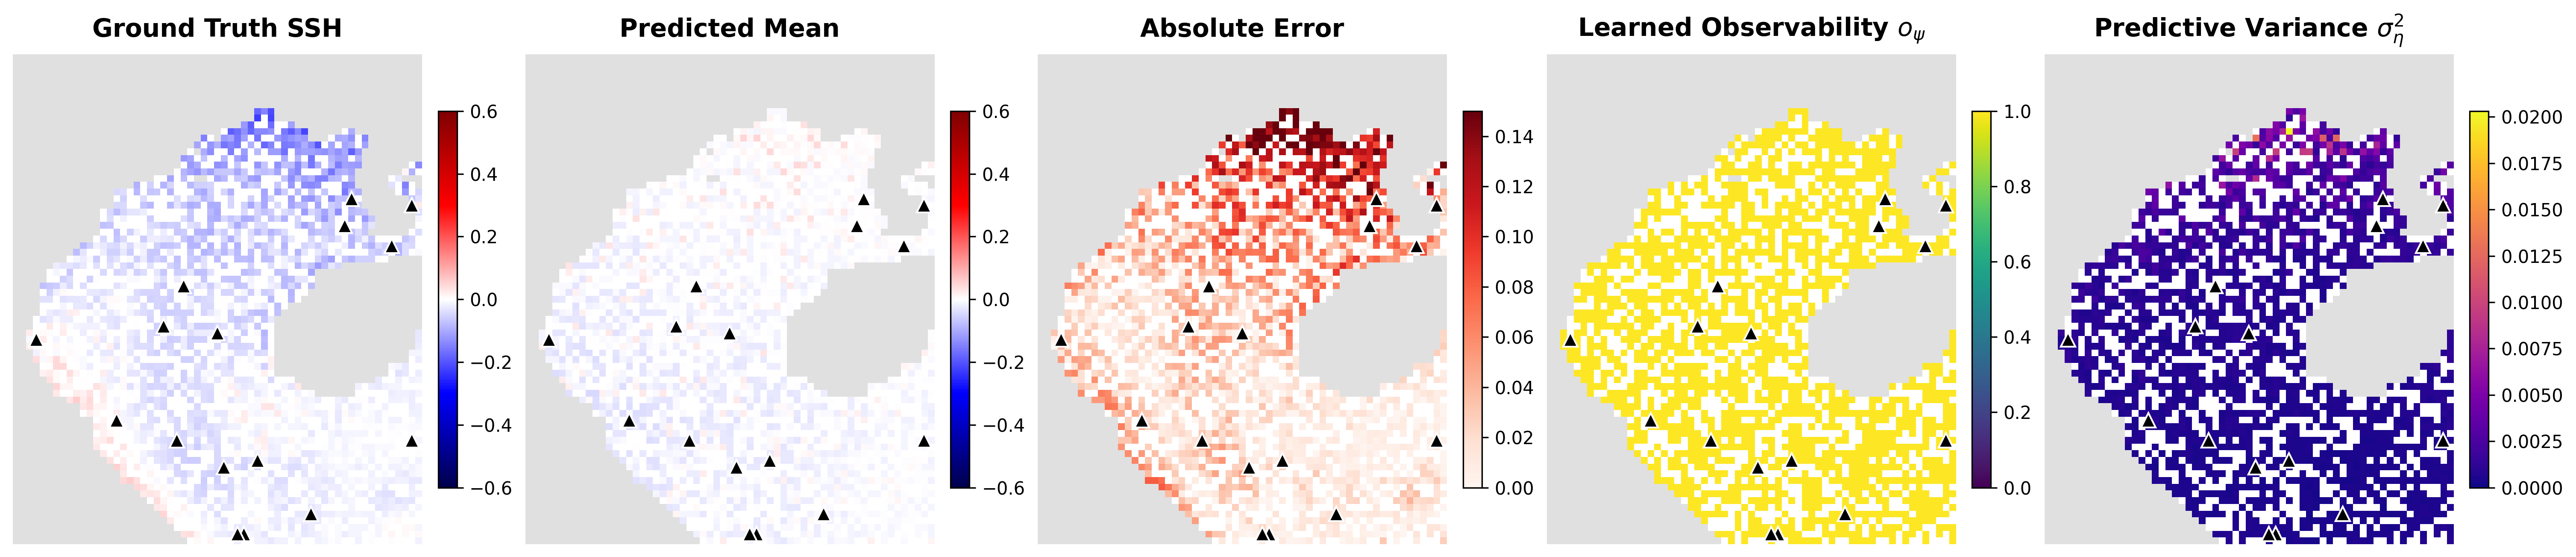
\includegraphics[width=\linewidth]{figures/observability_maps.png}
    \caption{Learned observability proxy on Copernicus SSH held-out validation data. From left to right: ground truth SSH, predicted mean, absolute error, learned observability score $o(x,y)$, and predictive variance. Regions with higher observability scores tend to exhibit lower error and lower predictive variance. The learned proxy is not supervised directly; it emerges from end-to-end training and is evaluated through its alignment with error and predictive variance (see Table~\ref{tab:obs_diagnostics}).}
    \label{fig:qualitative_copernicus}
\end{figure}

To further illustrate the temporal dynamics of the predictions, Figure~\ref{fig:forecast_trajectories} displays the continuous 1--24 h lead-time forecast trajectories at three representative locations covering different observability regimes.

\begin{figure}[!htbp]
    \centering
    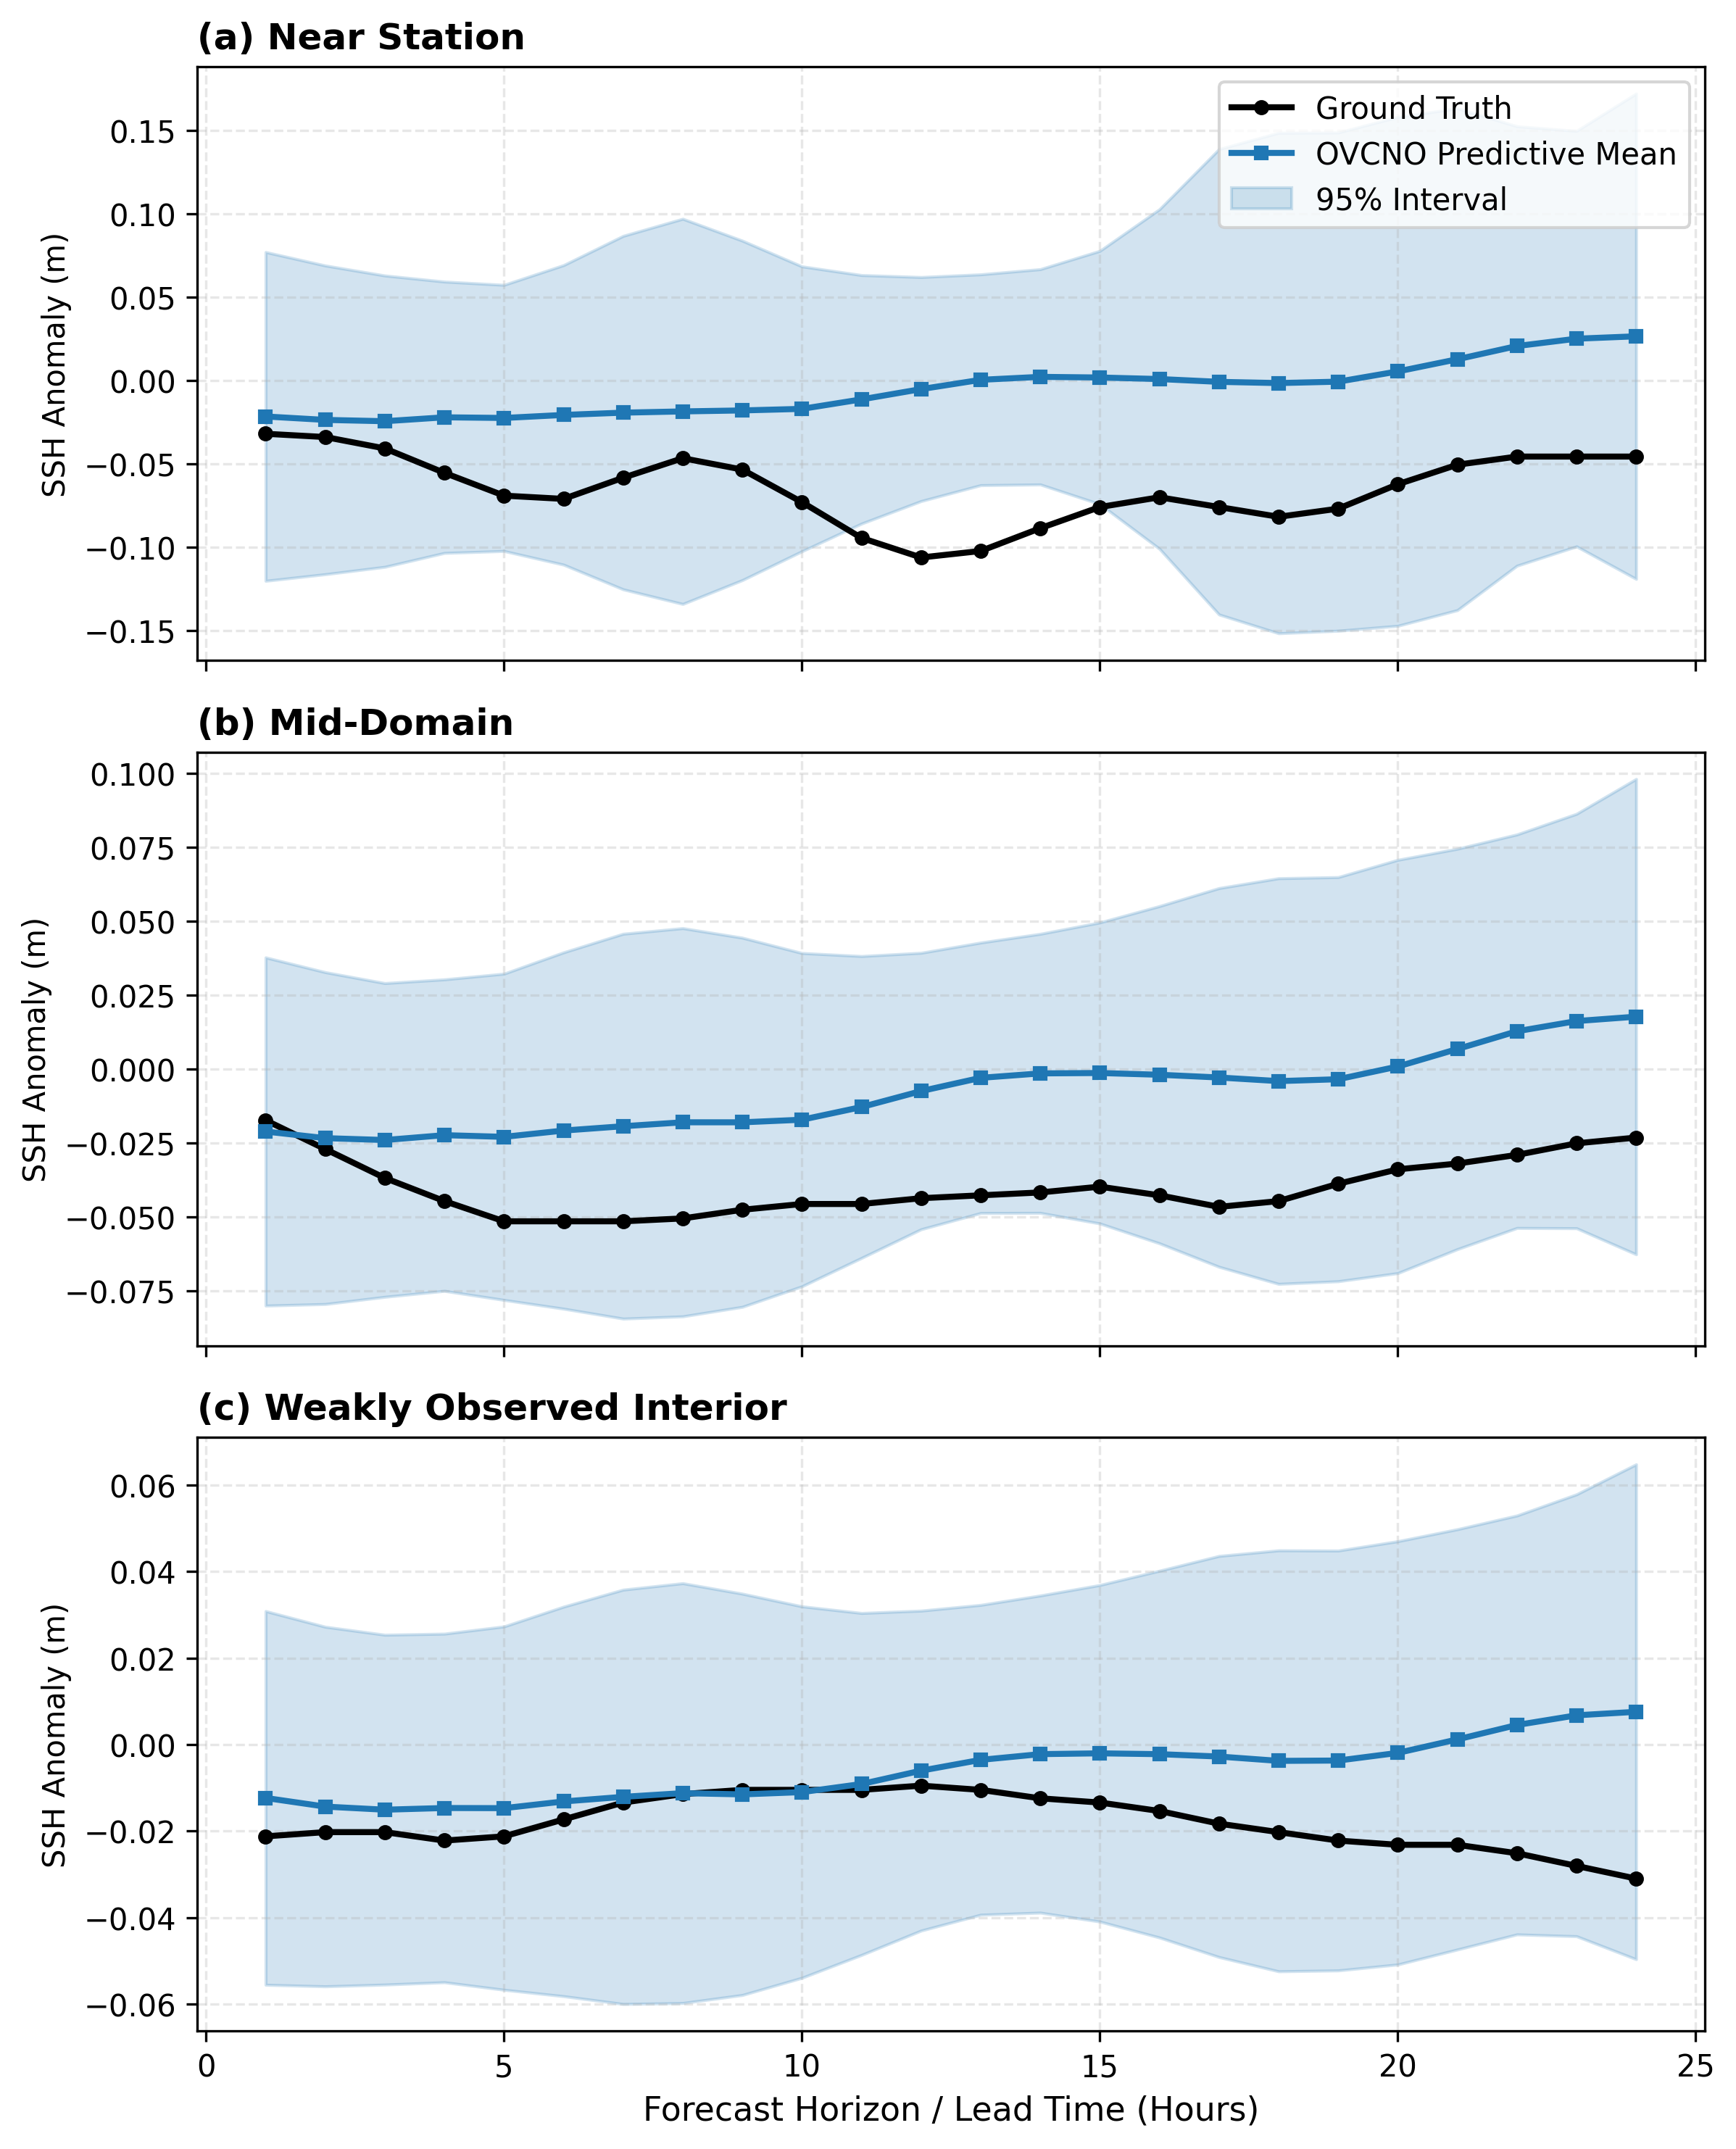
\includegraphics[width=0.85\linewidth]{figures/forecast_trajectories.png}
    \caption{Lead-time forecast trajectories at representative validation locations. The mean trajectory may exhibit visible bias at some locations, while the predictive intervals capture the realized trajectory and widen in weaker-observability regimes. This figure illustrates qualitative uncertainty behavior rather than trajectory-level accuracy. Values are shown in the same normalized SSH-anomaly scale used for evaluation.}
    \label{fig:forecast_trajectories}
\end{figure}

% -------------------------------------------------------------
\subsection{Ablation Studies}
\label{sec:ablation}
% -------------------------------------------------------------

\subsubsection{Component Ablation}

An ablation study examining the relative contributions of the sensor geometry encoder, the observability proxy, and the regularization components is provided in Appendix~\ref{app:ablation}. Due to stochasticity in training dynamics, the independently trained ablation runs exhibit shifted baseline metrics (e.g., larger average interval widths) compared to the main checkpoint presented in Table~\ref{tab:copernicus_results}. We therefore report them in the appendix to isolate relative component effects without conflating them with absolute headline performance.

\subsubsection{Observability Proxy Diagnostics}

To assess whether the learned observability score $o_\psi$ carries meaningful information about forecast difficulty, we compute diagnostic correlations between $o_\psi$ and both realized error $|e|$ and predictive standard deviation $\hat{\sigma}$.

\begin{table}[!htbp]
\centering
\caption{Observability-proxy diagnostics on Copernicus SSH validation data. Higher Pearson and Spearman correlations between the learned observability score and negated error/uncertainty indicate that the model tends to assign higher scores to better-observed regions.}
\label{tab:obs_diagnostics}
\vspace{4pt}
\begin{tabular}{@{}l c c@{}}
\toprule
\textbf{Diagnostic} & \textbf{OVCNO} & \textbf{OVCNO + adapt.~$\beta$} \\
\midrule
Pearson$(o_\psi, -|e|)$ & \textbf{0.221} & 0.101 \\
Pearson$(o_\psi, -\hat{\sigma})$ & \textbf{0.105} & 0.103 \\
Spearman$(o_\psi, -|e|)$ & \textbf{0.153} & 0.123 \\
Spearman$(o_\psi, -\hat{\sigma})$ & 0.121 & \textbf{0.134} \\
\bottomrule
\end{tabular}
\end{table}

The positive correlations indicate that regions assigned higher observability scores by the model tend to have lower forecast error and lower predictive uncertainty, consistent with the interpretation that $o_\psi$ serves as a data-driven observability proxy. The correlations are moderate rather than strong, reflecting the fact that $o_\psi$ is learned end-to-end without direct geometric supervision in the core OVCNO.


\subsubsection{Realistic Tide-Gauge Geometry OSSE}
\label{sec:real_geometry}

To move beyond synthetic equispaced boundary sensors, we introduce a real-station-geometry OSSE over the Gulf of Tonkin. We retain the same gridded ocean field, train/validation split, forecasting task, and OVCNO architecture as the main Copernicus SSH benchmark, but replace synthetic sensor locations with the coordinates of real coastal tide-gauge stations located within the model domain.

This is a Level-1 OSSE: station coordinates are taken from real coastal observing sites (sourced from PSMSL, IOC, and GLOSS databases), while sensor values are sampled from the gridded ocean analysis at the nearest valid ocean grid cell. This design isolates the effect of operational sensor geometry while preserving controlled full-field supervision. Figure~\ref{fig:station_map} shows the resulting station layout.

\begin{figure}[!htbp]
    \centering
    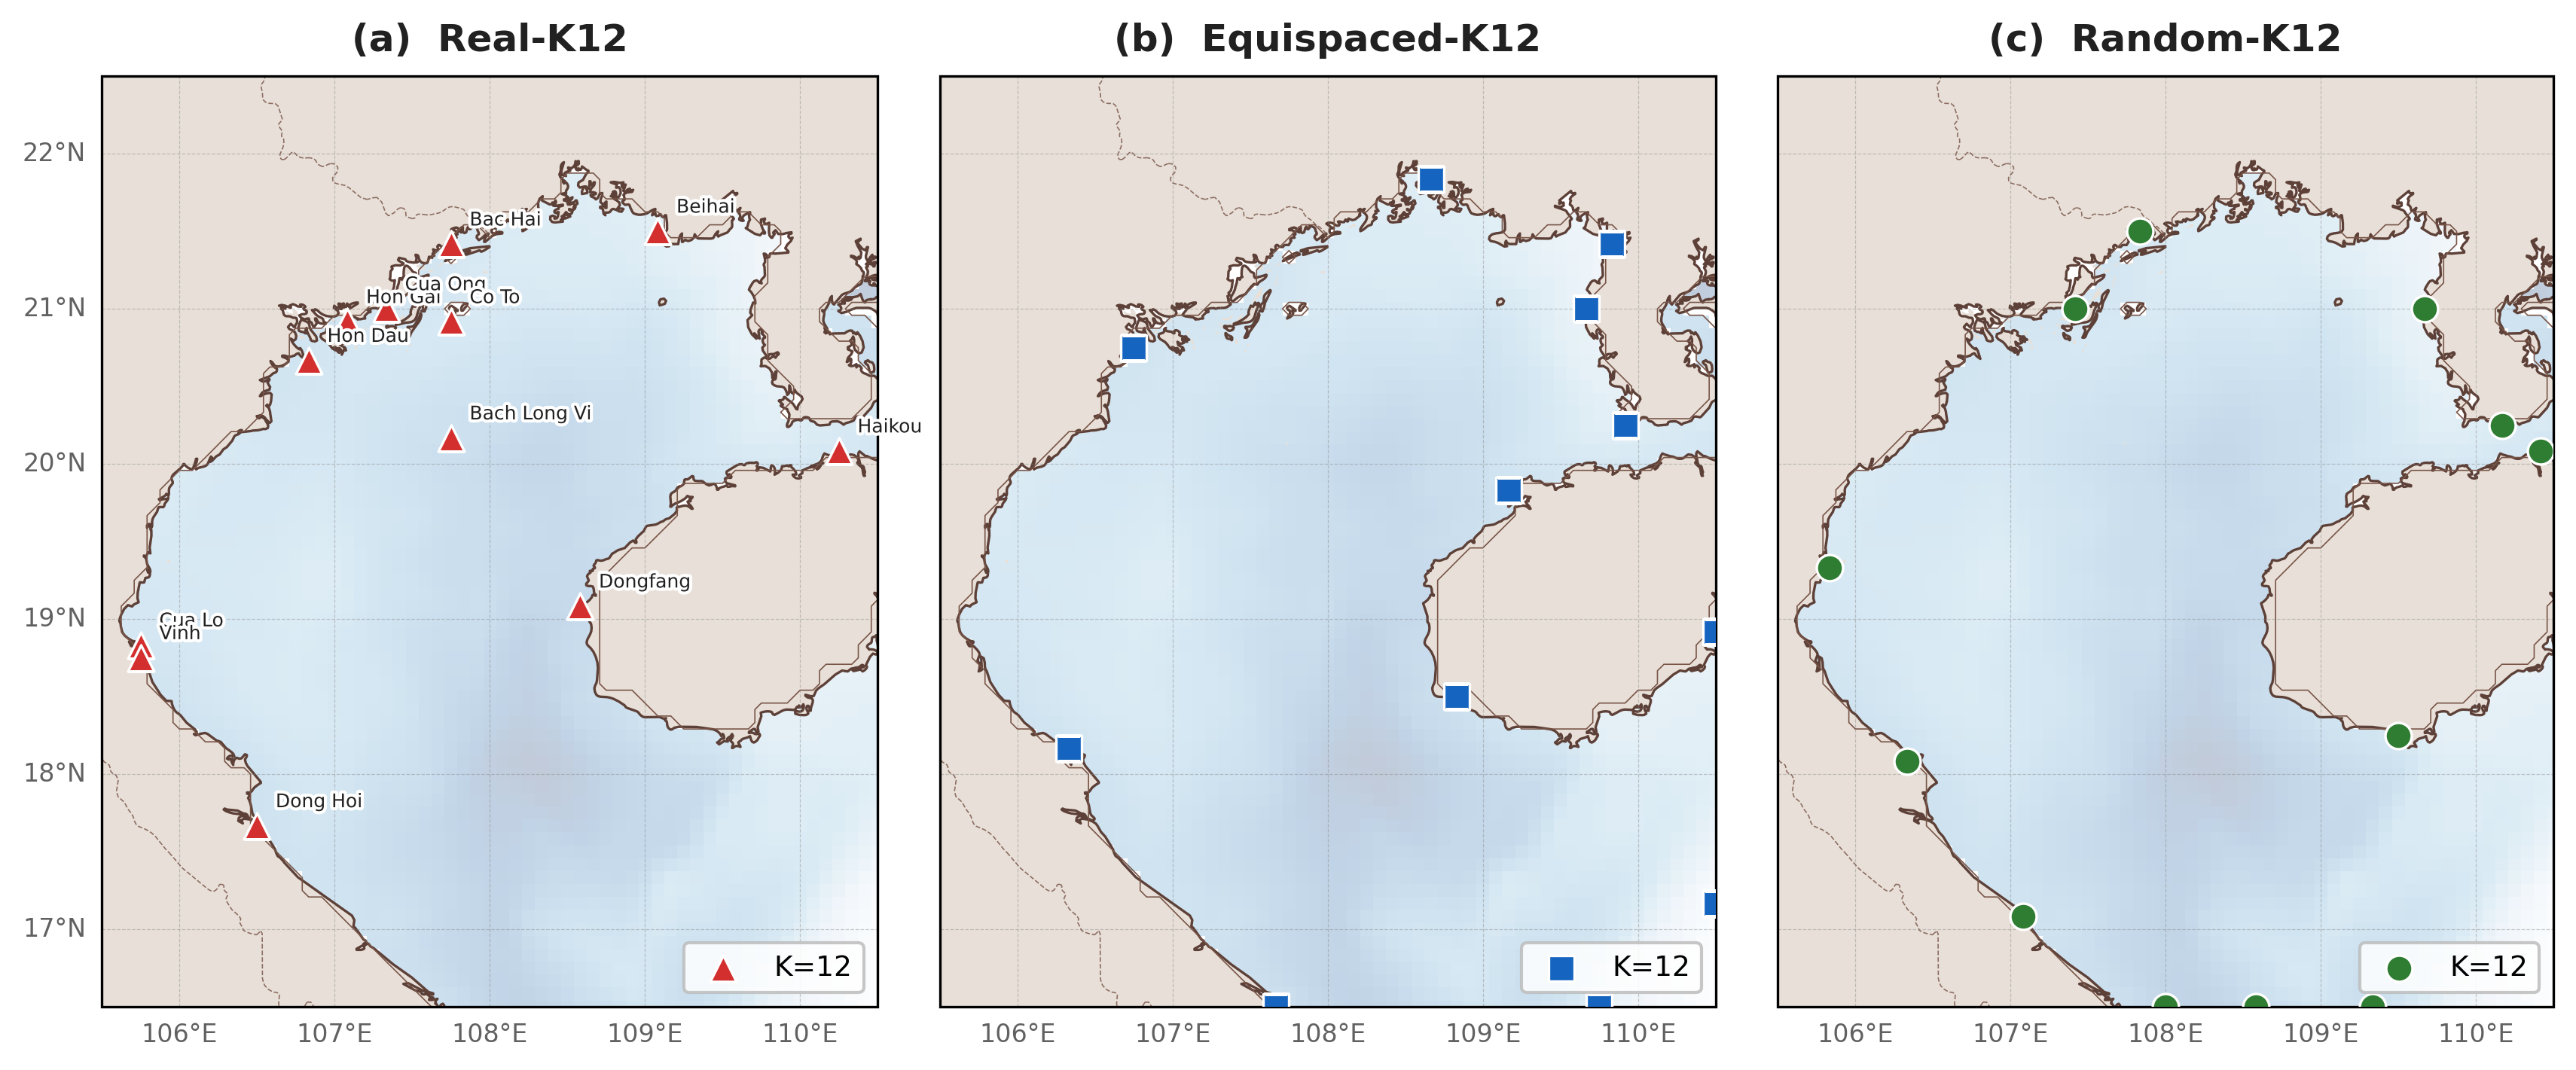
\includegraphics[width=\linewidth]{figures/layout_comparison.png}
    \caption{Sensor layouts used in the real-station-geometry OSSE. (A) Real-K12 exhibits operational redundancy and clustering near coastal stations. (B) Equispaced-K12 enforces uniform boundary spacing. (C) Random-K12 layouts are sampled from valid boundary points and used to estimate layout-induced variance under a fixed training seed.}
    \label{fig:station_map}
\end{figure}

We compare three sensor-layout families under the same fixed budget $K{=}12$: (i)~\textbf{Real-K12}, using real tide-gauge station geometry; (ii)~\textbf{Equispaced-K12}, using uniformly spaced boundary sensors; and (iii)~\textbf{Random-K12}, using randomly sampled boundary sensors. All models use the same architecture, optimizer, history length, forecast horizon, and query-point budget. Real-K12 and Equispaced-K12 are trained with 7 random seeds each; Random-K12 is evaluated over 5 random layouts with a fixed training seed. All normalization statistics (temporal mean subtraction) are computed on the training split only and reused unchanged for validation.

\begin{table}[!htbp]
\centering
\caption{Effect of sensor geometry under fixed budget $K{=}12$ (7-seed protocol). Real-K12 and Equispaced-K12 report mean$\pm$std across 7 training seeds; Random-K12 reports mean$\pm$std across 5 layout seeds with fixed training seed. These variances are therefore not directly interchangeable: the former measures training instability, the latter layout-induced variability. Note: the 7-seed pool here differs from the 3-seed subset used in Table~\ref{tab:missing_sensor}; numeric differences between the two tables (e.g., Corr$_S$ for Real-K12: 0.53 vs.\ 0.45) reflect different checkpoint populations rather than inconsistencies.}
\label{tab:real_geometry_osse}
\vspace{4pt}
\resizebox{\linewidth}{!}{
\begin{tabular}{@{}lccccccc@{}}
\toprule
\textbf{Layout} & $K$ & \textbf{RMSE}$\downarrow$ & \textbf{CRPS}$\downarrow$ & \textbf{Avg.W}$\downarrow$ & \textbf{Cov@95}$\uparrow$ & \textbf{NLL}$\downarrow$ & \textbf{Corr}$_S\!\uparrow$ \\
\midrule
Real-K12 & 12 & $0.065{\pm}.017$ & $0.035{\pm}.008$ & $0.254{\pm}.030$ & $94.6{\pm}6.6\%$ & $-1.40{\pm}.19$ & $0.53{\pm}.08$ \\
Equispaced-K12 & 12 & $0.061{\pm}.011$ & $0.034{\pm}.005$ & $0.278{\pm}.039$ & $96.8{\pm}5.0\%$ & $-1.42{\pm}.14$ & $0.50{\pm}.06$ \\
Random-K12 & 12 & $0.049{\pm}.001$ & $0.027{\pm}.000$ & $0.246{\pm}.007$ & $98.0{\pm}0.2\%$ & $-1.62{\pm}.02$ & $0.44{\pm}.01$ \\
\bottomrule
\end{tabular}}
\end{table}

The corrected results (with train-only normalization, latent sampling at evaluation, and full-grid spatial evaluation) do not support a clear point-accuracy advantage for any sensor layout at budget $K{=}12$. Because Random-K12 is evaluated across layout seeds under a fixed training seed, while Real-K12 and Equispaced-K12 are evaluated across training seeds, we do not interpret the lower Random-K12 mean RMSE as evidence of better layout geometry. Instead, training-seed variance dominates layout variance: Real-K12 and Equispaced-K12 exhibit RMSE standard deviations of 0.017 and 0.011, respectively, reflecting model initialization instability, while Random-K12 layouts show RMSE std of only 0.0005---a ratio of approximately 33:1. The main conclusion is that, at $K{=}12$, training initialization variance is a larger source of point-forecast variability than layout geometry. Figure~\ref{fig:topology_variance} visualizes the training-seed and layout-seed variance structure.

\begin{figure}[!htbp]
    \centering
    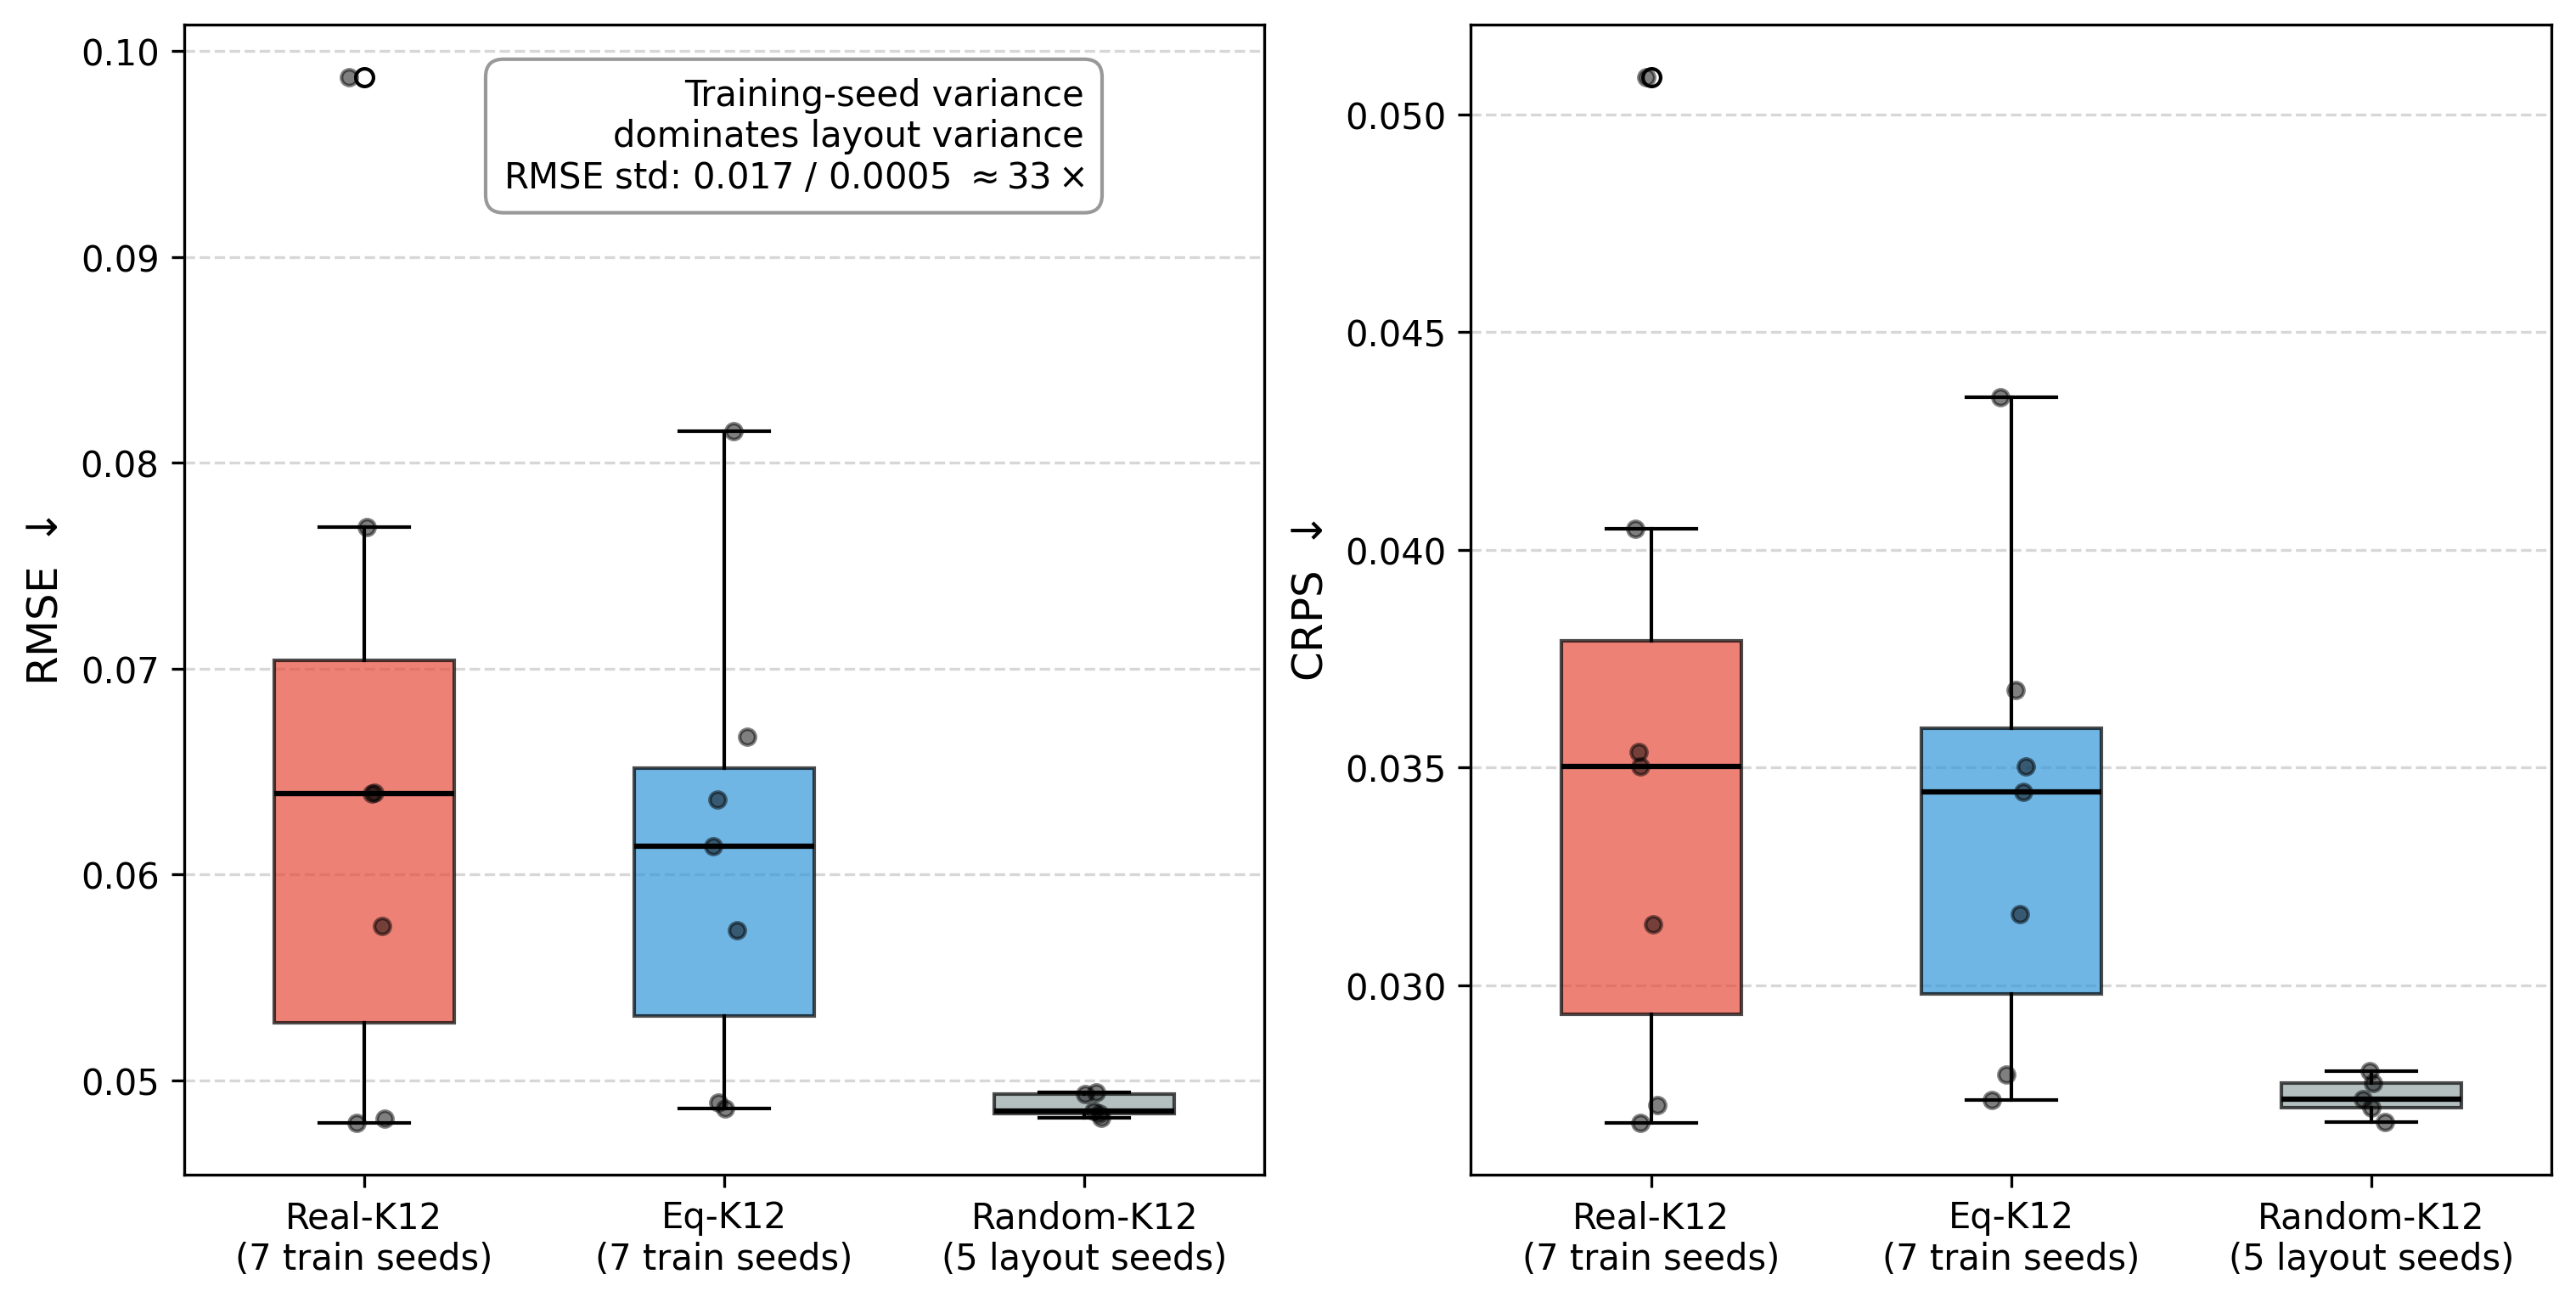
\includegraphics[width=0.85\linewidth]{figures/topology_variance.png}
    \caption{Variance structure in forecast quality under fixed $K{=}12$. Boxplots show the distribution of RMSE and CRPS for Real-K12 and Equispaced-K12 across 7 independent training seeds, compared to the distribution of Random-K12 across 5 different layout seeds under a single training seed. Under this protocol, training initialization variance is larger than the variance induced by layout geometry.}
    \label{fig:topology_variance}
\end{figure}

\paragraph{Missing-sensor robustness.}

Although point accuracy is comparable across layouts, sensor topology remains important for operational robustness under sensor outages. We evaluate each layout across 3 training seeds (42, 777, 2024) under sensor dropout at inference time, retaining 100\%, 75\%, and 50\% of sensors (10 random masks per level per seed).

\begin{table}[!htbp]
\centering
\caption{Missing-sensor robustness across 3 training seeds (seeds 42, 777, 2024---a subset of the 7-seed pool in Table~\ref{tab:real_geometry_osse}). Values at 100\% show mean$\pm$std across these 3 seeds; values at 75\%/50\% show mean$\pm$std across 3 seeds $\times$ 10 masks. Because this uses a different checkpoint subset than Table~\ref{tab:real_geometry_osse}, absolute metric values may differ. Evaluation uses all $\approx$2{,}520 ocean points.}
\label{tab:missing_sensor}
\vspace{4pt}
\begin{tabular}{@{}lccccccc@{}}
\toprule
\textbf{Layout} & \textbf{Avail.} & $K$ & \textbf{RMSE}$\downarrow$ & \textbf{CRPS}$\downarrow$ & \textbf{Avg.W}$\downarrow$ & \textbf{Cov@95}$\uparrow$ & \textbf{Corr}$_S\uparrow$ \\
\midrule
Real-K12 & 100\% & 12 & $0.051{\pm}.004$ & $0.029{\pm}.002$ & $0.259{\pm}.019$ & $98.8{\pm}0.6\%$ & $0.45{\pm}.04$ \\
Real-K12 & 75\% & 9 & $0.051{\pm}.004$ & $0.029{\pm}.002$ & $0.260{\pm}.023$ & $98.7{\pm}0.7\%$ & $0.45{\pm}.04$ \\
Real-K12 & 50\% & 6 & $0.051{\pm}.005$ & $0.029{\pm}.002$ & $0.261{\pm}.026$ & $98.7{\pm}0.8\%$ & $0.46{\pm}.04$ \\
\midrule
Eq-K12 & 100\% & 12 & $0.052{\pm}.004$ & $0.029{\pm}.002$ & $0.274{\pm}.020$ & $99.0{\pm}0.6\%$ & $0.47{\pm}.04$ \\
Eq-K12 & 75\% & 9 & $0.052{\pm}.004$ & $0.029{\pm}.002$ & $0.280{\pm}.015$ & $99.1{\pm}0.5\%$ & $0.47{\pm}.04$ \\
Eq-K12 & 50\% & 6 & $0.052{\pm}.004$ & $0.030{\pm}.002$ & $0.289{\pm}.003$ & $99.2{\pm}0.2\%$ & $0.47{\pm}.04$ \\
\bottomrule
\end{tabular}
\end{table}

Across training seeds and dropout masks, Real-K12 maintains nearly unchanged interval width under sensor dropout: mean Avg.W increases by only 0.8\% from 100\% to 50\% sensor availability (0.259$\to$0.261). In contrast, Equispaced-K12 exhibits a consistent widening pattern: mean Avg.W increases by 5.7\% from 0.274 to 0.289 at 50\% availability. RMSE remains comparable for both layouts across dropout levels, suggesting that the topology effect is primarily on uncertainty response rather than point accuracy.

\begin{figure}[!htbp]
    \centering
    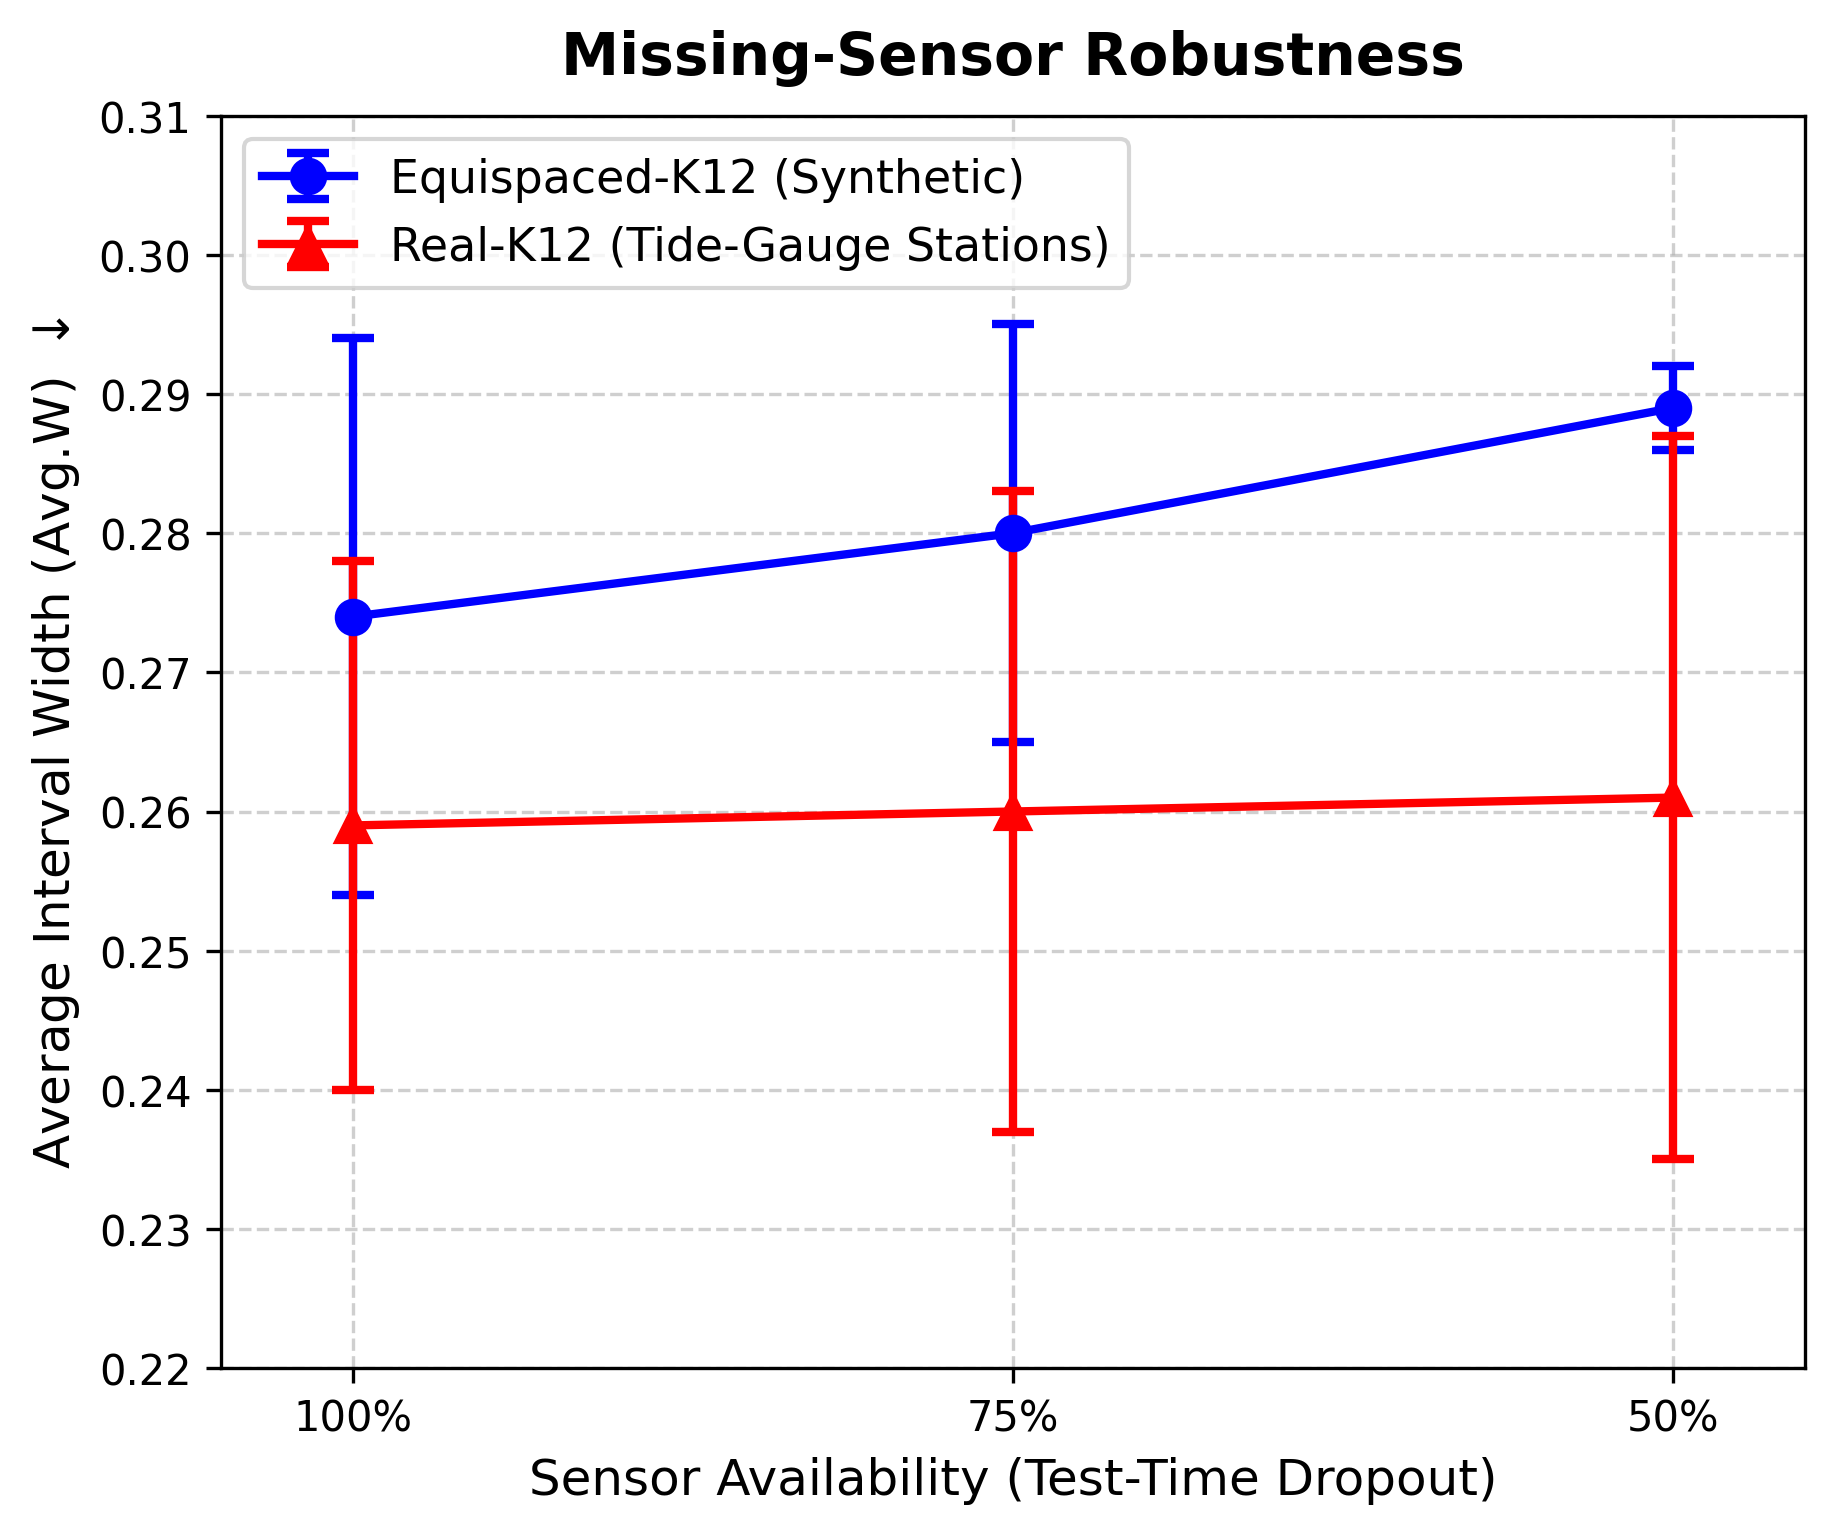
\includegraphics[width=0.55\linewidth]{figures/robustness_curve.png}
    \caption{Missing-sensor robustness under test-time sensor dropout. Real-K12 maintains nearly stable interval width as sensor availability decreases, while Equispaced-K12 exhibits systematic interval widening. This indicates that topology affects uncertainty robustness even when point RMSE remains comparable.}
    \label{fig:robustness_curve}
\end{figure}

Sensor topology thus appears to affect robustness and uncertainty response more than nominal point accuracy in this setting. The spatial redundancy present in the real station layout---particularly the adjacent Cua Lo and Vinh stations ($\sim$1 grid cell apart)---may provide more gradual degradation under sensor failure. Equispaced layouts lack this local redundancy, so each sensor dropout can create a larger observability gap. The set encoder enables inference with variable-size sensor sets without architectural changes; the empirical robustness, however, depends on the spatial redundancy of the retained sensors.

% -------------------------------------------------------------
\subsection{Observability and Uncertainty Analysis}
\label{sec:uncertainty_analysis}
% -------------------------------------------------------------

\subsubsection{Distance-Based Error Degradation}

To study how sparse observability affects prediction quality, we analyze forecasting error as a function of distance to the nearest observed boundary sensor. This experiment quantifies the extent to which interior regions become harder to forecast as they move farther away from direct observations.

\begin{figure}[!htbp]
    \centering
    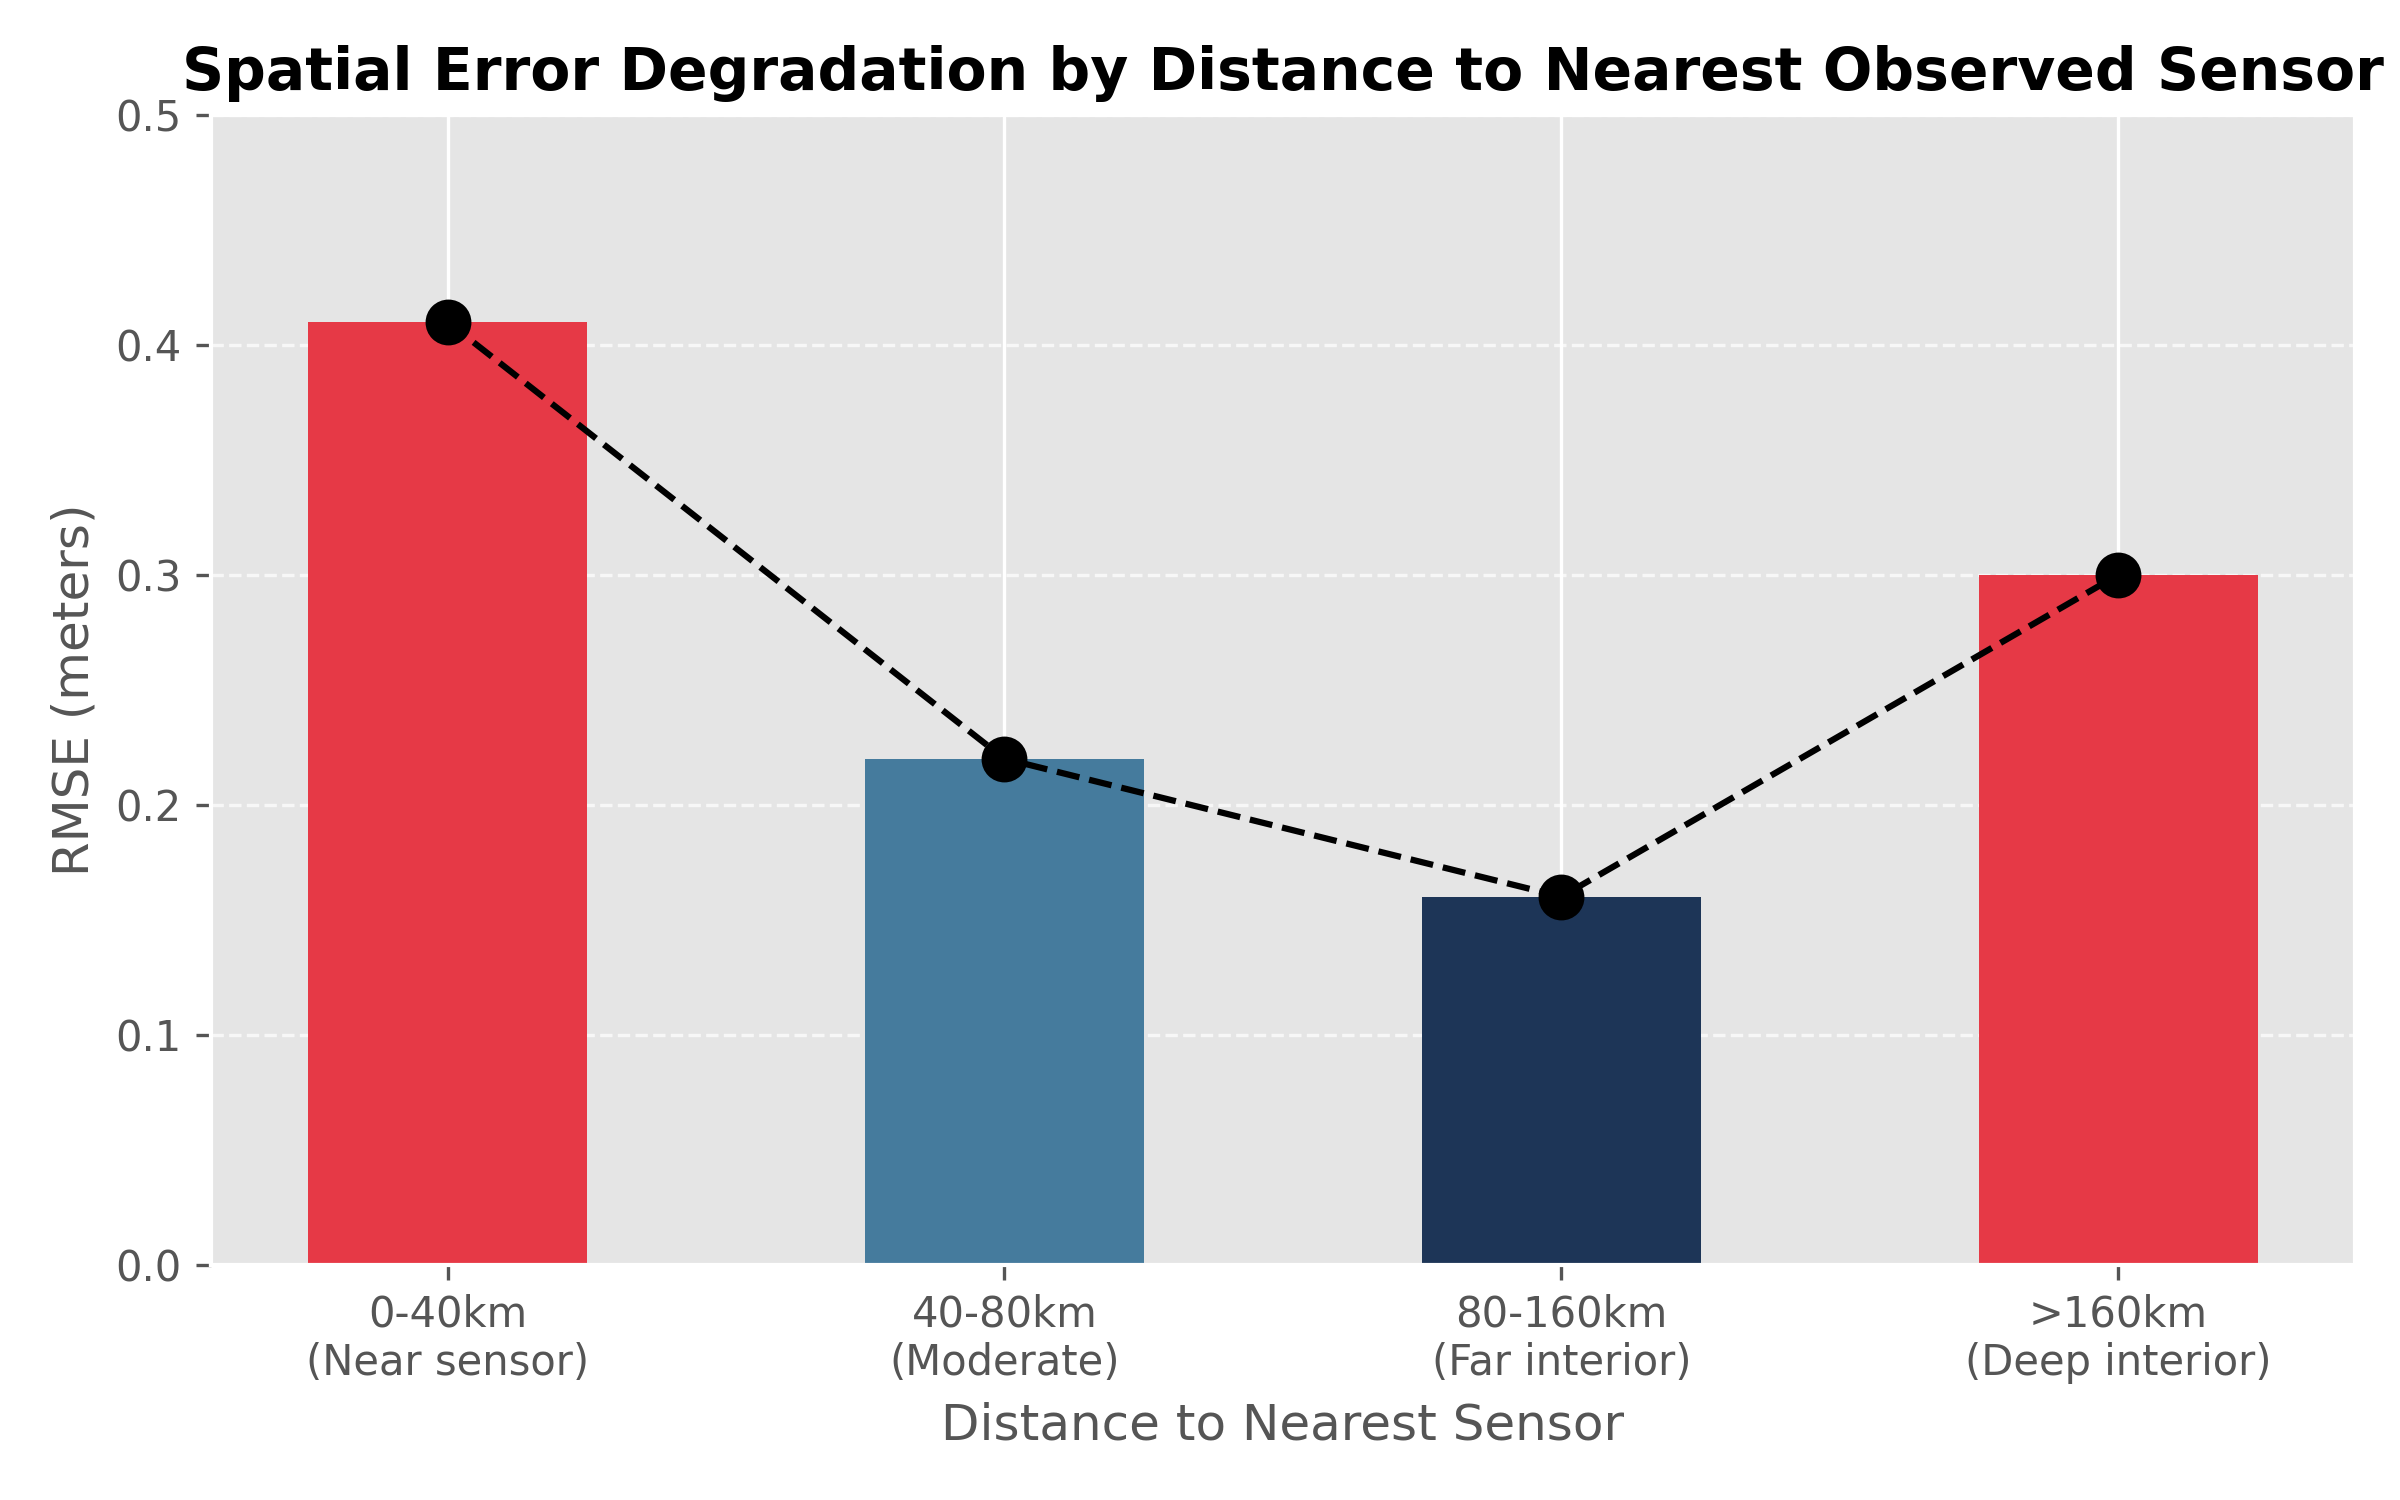
\includegraphics[width=0.72\linewidth]{figures/spatial_error_ushape.png}
    \caption{Forecasting error as a function of distance to the nearest observed sensor. The relationship is non-monotonic: both near-boundary regions (where coastal dynamics are complex) and far-interior regions (where observability is weakest) can exhibit elevated errors.}
    \label{fig:spatial_error}
\end{figure}

Prediction difficulty is spatially heterogeneous rather than simply increasing with distance. Both near-boundary dynamically active regions and far-interior weakly observed regions can exhibit elevated errors, producing a characteristic non-monotonic pattern. This suggests that a simple ``error increases with distance'' model is insufficient; the interplay between dynamical complexity and observability determines spatial forecast difficulty.

\subsubsection{Distance-Based Uncertainty Degradation}

We next analyze whether the predictive standard deviation produced by the proposed model follows the same observability trend. Figure~\ref{fig:uncertainty_distance} plots predictive standard deviation against distance to the nearest observed sensor.

\begin{figure}[!htbp]
    \centering
    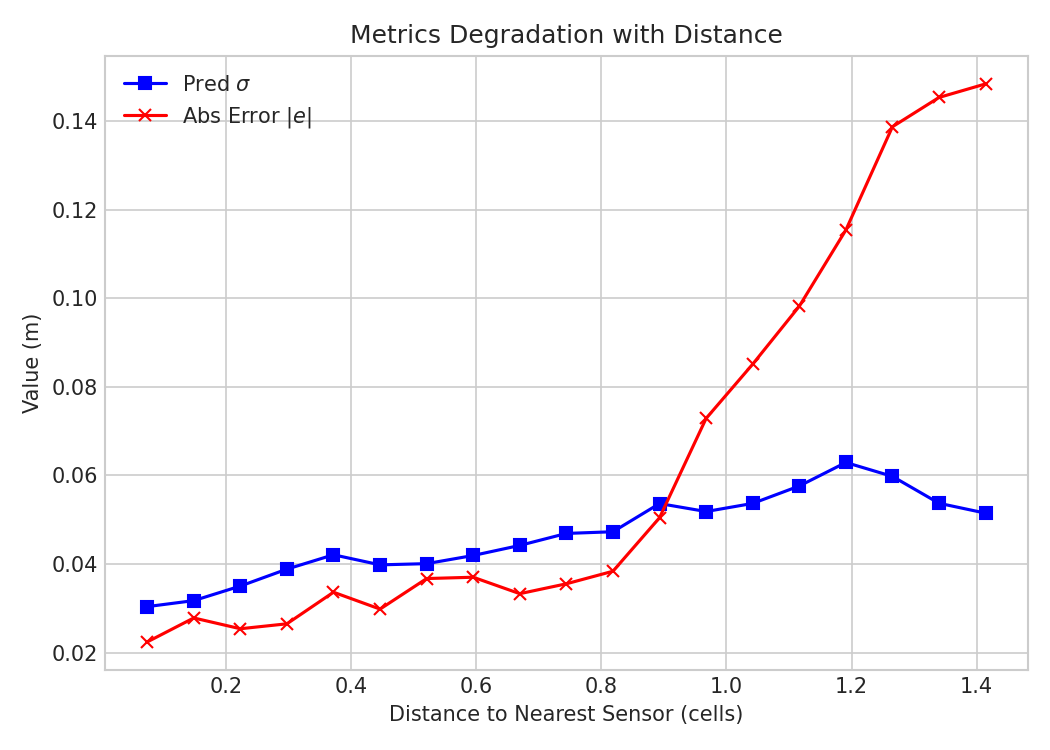
\includegraphics[width=0.72\linewidth]{figures/uncertainty_vs_distance.png}
    \caption{Predictive standard deviation $\hat{\sigma}$ as a function of distance to the nearest observed sensor. Higher uncertainty is generally associated with regions of weaker observability.}
    \label{fig:uncertainty_distance}
\end{figure}

Although the relationship is not perfectly monotonic at every individual query point, the overall trend shows that predictive uncertainty increases in poorly observed regions. This behavior is consistent with the view that sparse boundary measurements provide progressively weaker constraints on interior states as distance from the observed boundary increases.

\subsubsection{Error--Uncertainty Consistency}

A useful uncertainty estimate should correlate with actual forecasting difficulty. To test this, we compute the relationship between predicted standard deviation $\hat{\sigma}$ and absolute error $|e|$.

\begin{figure}[!htbp]
    \centering
    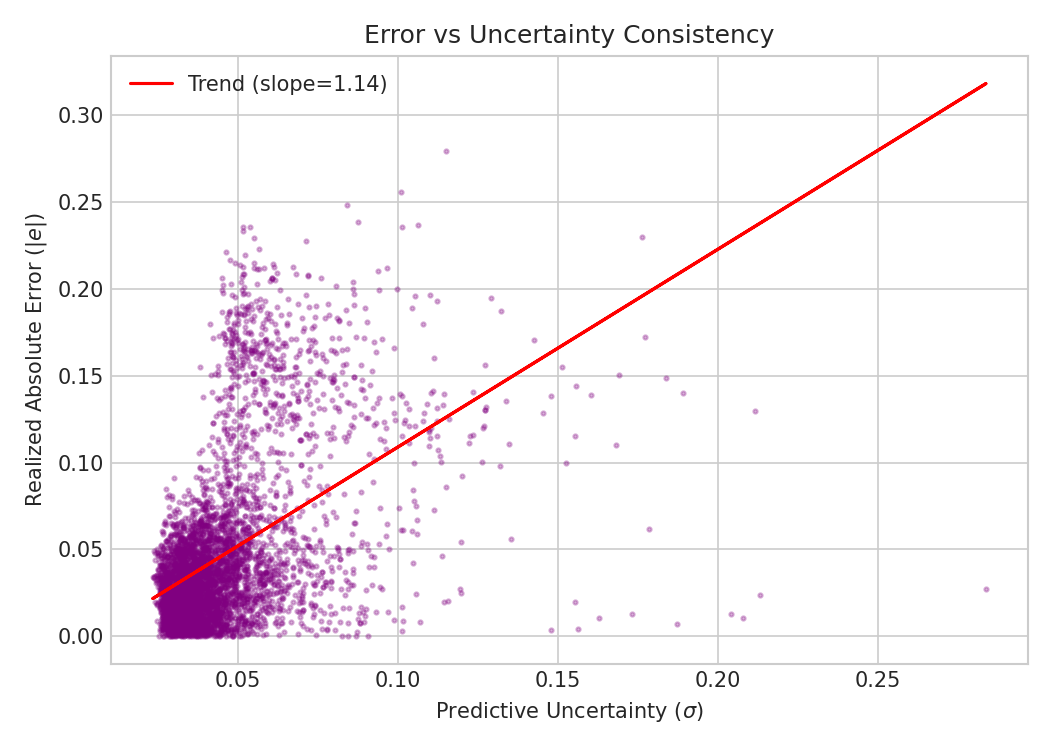
\includegraphics[width=0.72\linewidth]{figures/error_vs_uncertainty.png}
    \caption{Relationship between predictive uncertainty and realized absolute error.}
    \label{fig:error_uncertainty}
\end{figure}

We find that larger predictive uncertainty is associated with larger realized error, indicating that the uncertainty output is not merely an auxiliary parameter but carries meaningful information about forecast reliability.

\subsubsection{Calibration Analysis}

Finally, we evaluate probabilistic calibration using empirical interval coverage and reliability curves.

\begin{figure}[!htbp]
    \centering
    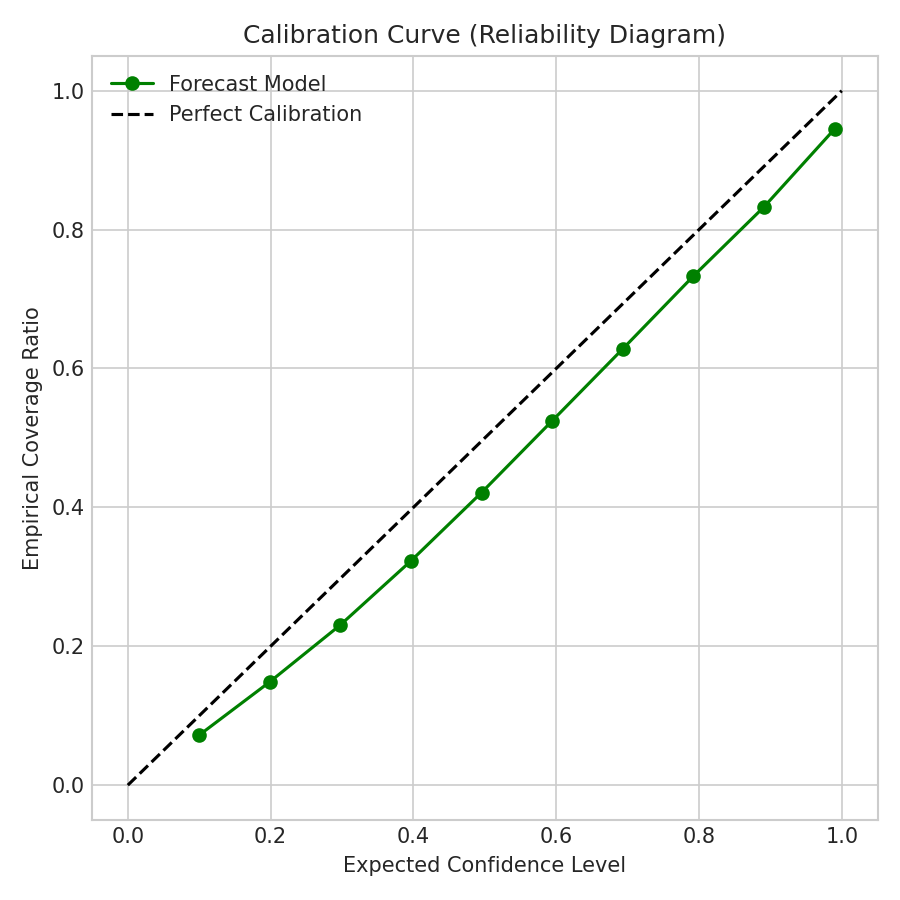
\includegraphics[width=0.72\linewidth]{figures/calibration_curve.png}
    \caption{Calibration analysis of the proposed probabilistic forecasts. Ideally, empirical coverage should closely match nominal coverage.}
    \label{fig:calibration_curve}
\end{figure}

The proposed model achieves near-nominal 95\% coverage (94.8\% vs.\ the nominal 95\%), indicating good calibration at the 95\% level. However, the reliability curve reveals that the model exhibits slight under-coverage at several lower nominal levels, suggesting that the Gaussian predictive distribution does not perfectly match the true residual distribution across all quantiles. As noted in Table~\ref{tab:copernicus_results}, coverage improvement comes with wider intervals (Avg.W = 0.287) compared with VCO (Avg.W = 0.209). Future work should investigate post-hoc calibration methods such as conformal prediction~\cite{feldman2023conformal} or recalibration to improve sharpness while maintaining reliable coverage.

\paragraph{Uncertainty sanity checks.}
To test whether the uncertainty--error correlation could be explained by mean-field collapse or distance-to-sensor confounding, we perform additional diagnostics on the Copernicus validation set (Table~\ref{tab:uncertainty_sanity}). The predicted mean exhibits no spatial collapse, with a spatial standard-deviation ratio of 1.54 relative to the ground truth. The Spearman correlation $\rho_S(|\varepsilon|,\hat{\sigma})$ remains high ($0.564$) after controlling for distance to the nearest sensor via partial correlation. Conditional Corr$_S$ remains positive on well-predicted samples ($0.272$) as well as poorly-predicted ones ($0.290$), suggesting that the alignment is not driven only by a small number of outliers. Finally, binning grid points by predicted $\hat{\sigma}$ into five equal-frequency quintiles yields a monotonic increase in MAE from $0.027$ in the lowest-uncertainty bin to $0.117$ in the highest-uncertainty bin. These checks support the interpretation that the learned uncertainty field carries information about forecast difficulty rather than merely reflecting sensor distance or a collapsed mean predictor.

\begin{table}[!htbp]
\centering
\caption{Uncertainty sanity checks for the proposed OVCNO on Copernicus validation data. These diagnostics test whether the reported uncertainty--error alignment is confounded by mean collapse, distance-to-sensor effects, or outlier-driven correlation.}
\label{tab:uncertainty_sanity}
\vspace{4pt}
\small
\begin{tabular}{@{}l c l@{}}
\toprule
\textbf{Diagnostic} & \textbf{Result} & \textbf{Interpretation} \\
\midrule
Spatial std.~ratio (pred / gt) & 1.54 & No mean collapse \\
Partial Corr$(|\varepsilon|,\hat{\sigma} \mid d_s)$ & 0.564 & Not explained by sensor distance alone \\
Good-sample Corr$_S$ & 0.272 & Persists on well-predicted samples \\
MAE by $\hat{\sigma}$ quintile & $0.027 \to 0.117$ & Monotonic risk stratification \\
\bottomrule
\end{tabular}
\end{table}


\subsection{Summary of Experimental Findings}

Across both controlled and ocean-analysis validation OSSE settings, the proposed OVCNO improves calibration, likelihood, CRPS, and risk localization relative to the VCO baseline, while paying a sharpness cost. The exploratory component ablation (Appendix~\ref{app:ablation}), which uses independently trained single-run variants rather than matched seeds, is indicative rather than conclusive and suggests the following trends:
\begin{enumerate}
    \item the sensor geometry encoder appears to be the largest contributor among the ablated variants, with an 18\% RMSE reduction and improved log-likelihood ($-1.92 \to -2.24$);
    \item the learned observability proxy further improves point accuracy and coverage in this set of variants, but produces wider intervals, suggesting a reliability--sharpness trade-off;
    \item the adaptive bottleneck improves sharpness relative to the proposed OVCNO, but reduces point accuracy and empirical coverage, suggesting a tunable coverage--sharpness trade-off;
    \item the main empirical gain appears to come from explicitly encoding sensor geometry and learning a query-dependent observability proxy, while additional regularization through adaptive KL weighting and ranking losses requires further investigation with matched-seed experiments;
    \item replacing synthetic equispaced sensors with real-station tide-gauge geometry shows that point accuracy is comparable across layouts at $K=12$, while training-seed variance dominates layout-induced variance;
    \item sensor topology primarily affects operational robustness under sensor dropout: real-station geometry maintains stable interval width, whereas equispaced layouts exhibit consistent interval widening.
\end{enumerate}

\section{Conclusion and Limitations}
\label{sec:conclusion}

We have presented OVCNO, a variational causal neural operator augmented with a \emph{learned observability proxy}---a data-driven score that estimates how strongly each spatial query point is constrained by the available sensor configuration. On a Copernicus SSH \emph{validation} OSSE over the Gulf of Tonkin (one-month chronological held-out period used for both evaluation and checkpoint selection, not a final independent test), OVCNO improves probabilistic forecast reliability relative to a VCO baseline: NLL from $-1.92$ to $-2.39$, CRPS from 0.043 to 0.036, empirical 95\% coverage from 79.7\% to 94.8\%, and Spearman error--uncertainty correlation from 0.446 to 0.523, while maintaining competitive point accuracy (RMSE 0.068 vs.\ 0.077). These gains come with moderately wider prediction intervals (Avg.W 0.209 $\to$ 0.287), reflecting a calibration--sharpness trade-off. The exploratory component ablation suggests that sensor geometry encoding is the largest contributor, while the learned observability proxy provides further calibration and coverage gains; however, these ablation conclusions are indicative rather than definitive, as the variants were trained as independent single runs rather than matched seeds.

The real-station-geometry OSSE further indicates that, at budget $K{=}12$, point accuracy is similar across Real-K12, Equispaced-K12, and Random-K12 layouts under the evaluated protocol, and training-seed variance is larger than layout-induced variance. Sensor topology remains relevant, however, for robustness under sensor outages: real-station geometry maintains stable interval width under 50\% sensor dropout, while equispaced layouts exhibit a widening in average interval width. These results suggest that evaluating observing networks should consider not only sensor count but also spatial redundancy and the induced constraint structure of the sensing geometry. Confirming these findings on independent multi-month test periods remains an important next step.

\textbf{Limitations.} Several limitations should be noted:
\begin{enumerate}
    \item \textbf{Calibration--sharpness trade-off.} OVCNO improves coverage, likelihood, and CRPS, but its intervals are wider than those of VCO (Avg.W 0.287 vs.\ 0.209). Improving sharpness while maintaining coverage---for example through conformal calibration~\cite{feldman2023conformal} or post-hoc recalibration---is an important direction.
    \item \textbf{Observability proxy.} The learned observability score $o_\psi$ is a data-driven proxy rather than a formal control-theoretic observability measure. Its correlations with error and uncertainty are positive but moderate, suggesting that explicit geometric or physics-informed supervision could further improve interpretability.
    \item \textbf{Level-1 OSSE only.} The real-station-geometry experiment uses real station coordinates but model-sampled sensor values, not actual tide-gauge observations. A Level-2 benchmark with real measurements, datum alignment, and withheld-station validation would strengthen operational deployment claims.
    \item \textbf{Validation rather than final test.} The present Copernicus benchmark is a controlled one-month OSSE designed to evaluate probabilistic sparse-sensor forecasting under a fixed protocol. Forecast targets are sampled over a uniformly distributed 1--24\,h lead-time window, with additional horizon-conditioned diagnostics reported at selected lead times. Metrics are reported on a chronological held-out period that is not used for gradient training, but the same period is also used for checkpoint selection. The reported numbers should therefore be interpreted as held-out validation performance, not as final test-set performance. A stronger operational benchmark would require multi-month or multi-season data, separate validation and test periods, and longer autoregressive rollouts.
    \item \textbf{Training stability.} The real-station-geometry OSSE reveals non-negligible training-seed variance, which can dominate layout-induced variance at the evaluated sensor budget. This limits the strength of conclusions about optimal sensor placement and motivates more stable training protocols, larger seed sweeps, and matched seed/layout experiments.
    \item \textbf{Mean--variance coupling.} The present decoder conditions both the predictive mean and variance on the learned observability proxy. Preliminary cross-product experiments on HYCOM revealed that product shifts can induce mean-collapse artifacts when the observability signal is coupled to both decoders simultaneously. Although Copernicus diagnostics show no such collapse in this study (spatial std ratio = 1.54), future work should investigate decoupled designs in which observability modulates only the variance pathway.
\end{enumerate}

\subsection*{Future Work}
\label{sec:future_work}

Several directions follow naturally from the limitations above and would strengthen the OVCNO framework from a controlled validation OSSE into an operational sparse-sensing forecasting system.

\paragraph{(i) Multi-month evaluation with independent test periods.}
The most immediate methodological gap is the use of a single-month chronological held-out window for both checkpoint selection and reporting (Limitation~4). We plan to extend the Copernicus benchmark to at least one full year of hourly SSH ($\geq$ 8{,}760 timesteps) and adopt a three-way temporal split, for example train Jan--Jul, validate on Aug, and report on Sep--Dec, so that none of the reported numbers can be attributed to selection bias. The same protocol would allow seasonal disaggregation (monsoon vs.\ inter-monsoon) and evaluation under storm or surge events, which exercise heavier-tailed residuals than the current January-only window.

\paragraph{(ii) Post-hoc calibration to recover sharpness.}
OVCNO improves coverage and likelihood at the cost of wider intervals (Limitation~1). A natural sharpening step is to apply distribution-free conformal calibration to the predictive intervals on a calibration set, then re-evaluate Cov@95\% and Avg.W on the test set. Both split conformal~\cite{angelopoulos2023conformal} and CQR-style approaches~\cite{romano2019cqr} are applicable here, and would allow OVCNO to retain the reliability gains observed in Table~\ref{tab:copernicus_results} while narrowing prediction intervals toward those of VCO.

\paragraph{(iii) Decoupled mean--variance architecture.}
The HYCOM cross-product investigation revealed that when the observability proxy $o_\psi$ feeds both the mean and variance heads, product shifts (Copernicus anomaly $\to$ HYCOM absolute SSH) can induce mean collapse with an artifactually high error--uncertainty correlation (Limitation~6). Although Copernicus diagnostics show no such collapse (spatial std ratio = 1.54), an architecture in which $o_\psi$ modulates only the variance pathway, while a separate mean decoder receives $z$ and $\phi(x,y,t)$ alone, would remove this failure mode by construction. A two-stage training schedule (first the mean head, then the variance head with the mean frozen) is a complementary mitigation. Both designs should be re-evaluated on HYCOM with the goal of recovering a non-collapsed mean predictor before attempting any cross-product reliability claim.

\paragraph{(iv) Level-2 OSSE with real tide-gauge measurements.}
Our real-station-geometry OSSE uses authentic station coordinates but model-sampled sensor values (Limitation~3). A Level-2 benchmark would replace these synthetic values with measured water-level time series from GLOSS, IOC Sea Level Station Monitoring Facility, or Copernicus Marine In~Situ TAC, after addressing datum alignment (chart datum vs.\ model reference), tidal harmonic alignment, and missing-data interpolation. To guard against the model simply re-fitting the gridded analysis, a subset of real gauges should be \emph{withheld at training and inference time} and used purely to evaluate predicted SSH at known operational locations.

\paragraph{(v) Cross-product and cross-region robustness.}
The current study evaluates a single product over a single coastal subdomain. Once decoupled mean--variance training (direction iii) is validated, we plan a controlled cross-product study comparing Copernicus CMEMS, HYCOM GOFS, and at least one operational forecasting system such as NOAA's CBOFS over an overlapping coastal domain (e.g.\ Chesapeake Bay, where dense tide-gauge networks make a parallel Level-2 protocol feasible). The metric of interest is not only RMSE but the stability of $o_\psi$ and Spearman Corr$(|\varepsilon|, \hat\sigma)$ across products, which would demonstrate whether observability-aware uncertainty is a transferable property of the architecture or an artifact of the original training distribution.

\paragraph{(vi) Matched-seed ablations and sensor-placement sweeps.}
The component ablation in Appendix~\ref{app:ablation} consists of independently trained single runs and is therefore indicative rather than conclusive. A matched-seed ablation, in which each variant is trained from the same 5--7 random seeds with all other settings fixed, would convert the appendix into a defensible quantitative contribution. The same multi-seed protocol should be applied to the sensor-placement experiment (Section~\ref{sec:real_geometry}), where the current training-seed variance dominates layout-induced variance at $K{=}12$; sweeping $K \in \{8, 16, 24, 32\}$ with matched seeds would let us isolate when (and whether) observability geometry becomes the dominant factor.

\paragraph{(vii) Explicit supervision of the observability proxy.}
The learned $o_\psi$ emerges from end-to-end training and exhibits only moderate correlations with absolute error (Pearson $\approx 0.22$) and predictive variance (Pearson $\approx 0.11$); see Table~\ref{tab:obs_diagnostics}. A natural enhancement is to add a weak supervisory signal derived either from a control-theoretic observability Gramian on a linearized surrogate dynamics, from a physics-informed information-flow proxy, or from cross-validation residuals on withheld sensors. Such supervision would let us test whether explicit geometric priors can sharpen the proxy without sacrificing the data-driven flexibility that allows it to adapt to heterogeneous coastal dynamics.

\paragraph{(viii) Longer autoregressive horizons and multi-variable extension.}
The current evaluation reports lead times of 1--24~hours with single-step query forecasts. Operational coastal forecasting typically requires multi-day rollouts and joint prediction of SSH, surface currents, and water temperature. Extending OVCNO to autoregressive forecasting (re-encoding predicted states as pseudo-observations) and to a multi-variable decoder is straightforward in principle but raises new questions about uncertainty accumulation, observability decay over rollouts, and whether the observability proxy can meaningfully discriminate between variables that share the same sensor budget.

Taken together, directions~(i)--(iii) address the three most pressing methodological gaps in the present paper and are the highest-priority next steps. Directions~(iv)--(viii) outline a path toward an operational-grade sparse-sensing forecasting system with transferable, interpretable, and physically grounded observability awareness.

\begin{thebibliography}{20}
% ══════════════════════════════════════════════════════════════

\bibitem{li2021fno}
Z.~Li, N.~Kovachki, K.~Azizzadenesheli, B.~Liu, K.~Bhatt, A.~Stuart, and A.~Anandkumar,
``Fourier Neural Operator for Parametric Partial Differential Equations,''
in \textit{Proc.\ ICLR}, 2021.

\bibitem{lu2021deeponet}
L.~Lu, P.~Jin, G.~Pang, Z.~Zhang, and G.~E.~Karniadakis,
``Learning nonlinear operators via DeepONet based on the universal approximation theorem of operators,''
\textit{Nature Machine Intelligence}, vol.~3, no.~3, pp.~218--229, 2021.
doi: \href{https://doi.org/10.1038/s42256-021-00302-5}{10.1038/s42256-021-00302-5}.

\bibitem{raissi2019pinns}
M.~Raissi, P.~Perdikaris, and G.~E.~Karniadakis,
``Physics-informed neural networks: A deep learning framework for solving forward and inverse problems involving nonlinear partial differential equations,''
\textit{Journal of Computational Physics}, vol.~378, pp.~686--707, 2019.
doi: \href{https://doi.org/10.1016/j.jcp.2018.10.045}{10.1016/j.jcp.2018.10.045}.

\bibitem{wang2021pideeponet}
S.~Wang, H.~Wang, and P.~Perdikaris,
``Learning the solution operator of parametric partial differential equations with physics-informed DeepONets,''
\textit{Science Advances}, vol.~7, no.~40, article eabi8605, 2021.
doi: \href{https://doi.org/10.1126/sciadv.abi8605}{10.1126/sciadv.abi8605}.

\bibitem{takamoto2022pdebench}
M.~Takamoto, T.~Praditia, R.~Leiteritz, D.~MacKinlay, F.~Alesiani, D.~Pfl\"{u}ger, and M.~Niepert,
``PDEBench: An Extensive Benchmark for Scientific Machine Learning,''
in \emph{Advances in Neural Information Processing Systems (NeurIPS)}, 2022.

\bibitem{rahman2024codano}
M.~A.~Rahman, R.~J.~George, M.~Elleithy, D.~Leibovici, Z.~Li, B.~Bonev, C.~White, J.~Berner, R.~A.~Yeh, J.~Kossaifi, K.~Azizzadenesheli, and A.~Anandkumar,
``Pretraining Codomain Attention Neural Operators for Solving Multiphysics PDEs,''
in \emph{Advances in Neural Information Processing Systems (NeurIPS)}, 2024.
Also available as \emph{arXiv:2403.12553}.

\bibitem{liu2026physics}
X.~Liu and Y.~G.~Lai,
``Physics-Informed Deep Operator Learning for Computational Hydraulics Modeling,''
\emph{arXiv:2601.08086}, 2026.

\bibitem{loshchilov2019adamw}
I.~Loshchilov and F.~Hutter,
``Decoupled Weight Decay Regularization,''
in \textit{Proc.\ ICLR}, 2019.

\bibitem{nguyen2009godunov}
T.~T.~Nguyen and T.~H.~Nguyen,
``Application of a Godunov type numerical scheme and a domain decomposition technique to the parallel computation of tidal propagation,''
\textit{VNU J.\ Sci., Earth Sci.}, vol.~25, pp.~104--115, 2009.

\bibitem{hendrycks2016gelu}
D.~Hendrycks and K.~Gimpel,
``Gaussian Error Linear Units (GELUs),''
\textit{arXiv:1606.08415}, 2016.

\bibitem{xu2024coastal}
Z.~Xu, J.~Ren, Y.~Zhang, J.~M.~G.~Ondina, M.~Olabarrieta, T.~Xiao, W.~He, Z.~Liu, S.~Chen, K.~Smith, and Z.~Jiang,
``A Fast AI Surrogate for Coastal Ocean Circulation Models,''
\emph{arXiv:2410.14952}, 2024.

\bibitem{zaheer2017deepsets}
M.~Zaheer, S.~Kottur, S.~Ravanbakhsh, B.~Poczos, R.~Salakhutdinov, and A.~Smola,
``Deep Sets,''
in \emph{Advances in Neural Information Processing Systems (NeurIPS)}, 2017.

\bibitem{kingma2013vae}
D.~P.~Kingma and M.~Welling,
``Auto-Encoding Variational Bayes,''
in \emph{Proc.\ ICLR}, 2014.

\bibitem{gneiting2007calibration}
T.~Gneiting, F.~Balabdaoui, and A.~E.~Raftery,
``Probabilistic forecasts, calibration and sharpness,''
\textit{Journal of the Royal Statistical Society: Series B}, vol.~69, no.~2, pp.~243--268, 2007.
doi: \href{https://doi.org/10.1111/j.1467-9868.2007.00587.x}{10.1111/j.1467-9868.2007.00587.x}.

\bibitem{lellouche2018cmems}
J.-M.~Lellouche, E.~Greiner, O.~Le~Galloudec, G.~Garric, C.~Regnier, M.~Drevillon, M.~Benkiran, C.-E.~Testut, R.~Bourdalle-Badie, F.~Gasparin, O.~Hernandez, B.~Levier, Y.~Drillet, E.~Remy, and P.-Y.~Le~Traon,
``Recent updates to the Copernicus Marine Service global ocean monitoring and forecasting real-time $1/12^\circ$ high-resolution system,''
\textit{Ocean Science}, vol.~14, pp.~1093--1126, 2018.
doi: \href{https://doi.org/10.5194/os-14-1093-2018}{10.5194/os-14-1093-2018}.

\bibitem{fablet2021learning}
R.~Fablet, B.~Chapron, L.~Drumetz, E.~M\'{e}min, O.~Pannekoucke, and F.~Rousseau,
``Learning variational data assimilation models and solvers,''
\textit{Journal of Advances in Modeling Earth Systems}, vol.~13, article e2021MS002572, 2021.
doi: \href{https://doi.org/10.1029/2021MS002572}{10.1029/2021MS002572}.

\bibitem{psaros2023uncertainty}
A.~F.~Psaros, X.~Meng, Z.~Zou, L.~Guo, and G.~E.~Karniadakis,
``Uncertainty quantification in scientific machine learning: Methods, metrics, and comparisons,''
\textit{Journal of Computational Physics}, vol.~477, article 111902, 2023.
doi: \href{https://doi.org/10.1016/j.jcp.2022.111902}{10.1016/j.jcp.2022.111902}.

\bibitem{yin2023dino}
Y.~Yin, M.~Kirchmeyer, J.-Y.~Franceschi, A.~Rakotomamonjy, and P.~Gallinari,
``Continuous PDE Dynamics Forecasting with Implicit Neural Representations,''
in \emph{Proc.\ ICLR}, 2023.

\bibitem{herde2024poseidon}
M.~Herde, B.~Raoni\'{c}, T.~Rohner, R.~K\"{a}ppeli, R.~Molinaro, E.~de~B\'{e}zenac, and S.~Mishra,
``Poseidon: Efficient Foundation Models for PDEs,''
in \emph{Advances in Neural Information Processing Systems (NeurIPS)}, 2024.
Also available as \emph{arXiv:2405.19101}.
% Note: cited as foundation model for PDE operators.

\bibitem{feldman2023conformal}
S.~Feldman, S.~Bates, and Y.~Romano,
``Calibrated Multiple-Output Quantile Regression with Representation Learning,''
\textit{J.\ Mach.\ Learn.\ Res.}, vol.~24, no.~24, pp.~1--48, 2023.
% Note: uses conformal prediction for calibrated multivariate prediction regions.

\bibitem{santos2023senseiver}
J.~E.~Santos, Z.~R.~Fox, A.~Mohan, D.~O'Malley, H.~Viswanathan, and N.~Lubbers,
``Development of the Senseiver for efficient field reconstruction from sparse observations,''
\textit{Nature Machine Intelligence}, vol.~5, pp.~1317--1325, 2023.
doi: \href{https://doi.org/10.1038/s42256-023-00746-x}{10.1038/s42256-023-00746-x}.

\bibitem{moya2024conformal}
C.~Moya, A.~Mollaali, Z.~Zhang, L.~Lu, and G.~Lin,
``Conformalized-DeepONet: A Distribution-Free Framework for Uncertainty Quantification in Deep Operator Networks,''
\emph{arXiv:2402.15406}, 2024.

\bibitem{angelopoulos2023conformal}
A.~N.~Angelopoulos and S.~Bates,
``Conformal Prediction: A Gentle Introduction,''
\textit{Foundations and Trends in Machine Learning}, vol.~16, no.~4, pp.~494--591, 2023.
doi: \href{https://doi.org/10.1561/2200000101}{10.1561/2200000101}.

\bibitem{romano2019cqr}
Y.~Romano, E.~Patterson, and E.~J.~Cand\`{e}s,
``Conformalized Quantile Regression,''
in \emph{Advances in Neural Information Processing Systems (NeurIPS)}, 2019.

\end{thebibliography}

\appendix
\section{Component Ablation Study}
\label{app:ablation}

To explore the contribution of individual OVCNO components, we trained five model variants on the Copernicus SSH benchmark. Because each variant is trained independently as a single run without matched seeds, the training landscape exhibits non-negligible run-to-run variance, and the ablation variants exhibit shifted baseline metrics compared to the main checkpoint in Table~\ref{tab:copernicus_results}. \textbf{Importantly, the ablation OVCNO row here is a different run from the headline OVCNO in Table~\ref{tab:copernicus_results}}: it achieves lower RMSE (0.0619 vs.\ 0.0683) but much wider intervals (Avg.W 0.572 vs.\ 0.287), illustrating the degree to which single-run stochasticity can shift the calibration--sharpness operating point. The headline checkpoint was selected by validation NLL from a separate training run. For this reason, these results are \emph{indicative} rather than conclusive, and should be used to understand qualitative component trends rather than to make precise quantitative claims. The regularization rows should be read as exploratory variants, not as improvements over the proposed headline model. A matched-seed ablation study would strengthen these observations and is left for future work.

\begin{table}[!htbp]
\centering
\caption{Component ablation on Copernicus SSH (\textbf{indicative, not conclusive}: each variant is an independent single-run without matched seeds). OVCNO-Geom adds the sensor geometry encoder; OVCNO further adds the learned observability proxy. The last two rows are exploratory regularization variants.}
\label{tab:ovcno_ablation_app}
\vspace{4pt}
\small
\resizebox{\linewidth}{!}{
\begin{tabular}{@{}l cccccc@{}}
\toprule
\textbf{Variant} & \textbf{RMSE}$\downarrow$ & \textbf{NLL}$\downarrow$ & \textbf{CRPS}$\downarrow$ & \textbf{Avg.W}$\downarrow$ & \textbf{Cov@95\%} & \textbf{Corr}$_S\!\uparrow$ \\
\midrule
VCO baseline & 0.0765 & $-1.92$ & \textbf{0.043} & \textbf{0.209} & 79.7\% & 0.446 \\
OVCNO-Geom (+ geom.~enc.) & 0.0629 & $-2.24$ & 0.042 & 0.505 & 97.8\% & 0.534 \\
\textbf{OVCNO (+ obs.~proxy)} & \textbf{0.0619} & \textbf{$-2.19$} & 0.045 & 0.572 & \textbf{98.7\%} & 0.514 \\
\midrule
\multicolumn{7}{@{}l}{\textit{Regularization extensions}}\\
OVCNO + adaptive $\beta$ & 0.0876 & $-2.23$ & 0.044 & 0.322 & 92.4\% & \textbf{0.634} \\
OVCNO + adapt.~$\beta$ + rank & 0.0779 & $-2.22$ & 0.041 & 0.273 & 91.9\% & 0.572 \\
\bottomrule
\end{tabular}}
\end{table}

The ablation is indicative of two qualitative trends. First, the \textbf{sensor geometry encoder appears to provide the largest improvement in this set of variants}: RMSE drops from 0.0765 to 0.0629 (an 18\% reduction), coverage increases from 80\% to 98\%, and the predictive log-likelihood improves ($-1.92 \to -2.24$). This is suggestive of the importance of encoding sensor locations alongside their values for spatial uncertainty awareness, though the magnitude of the effect should be confirmed with matched-seed experiments.

Second, the structural additions appear to introduce a reliability--sharpness trade-off. The core OVCNO components (geometry + observability proxy) yield strong likelihood and coverage but produce conservative intervals (Avg.W = 0.572). The adaptive bottleneck tightens these intervals, reducing Avg.W to 0.322 and CRPS to 0.044, though at the cost of lower coverage and worse RMSE. The ranking loss further narrows intervals (Avg.W = 0.273) with a moderate improvement in RMSE relative to the adaptive-$\beta$ variant, but neither regularized variant dominates the proposed headline model. These exploratory results suggest that regularization can tune interval sharpness, but also introduces optimization and point-accuracy trade-offs that warrant further investigation.

\section{Additional Ablations: Sensor Budget}
\label{app:sensor_budget}

We also vary the number of boundary sensors to evaluate how predictive performance and uncertainty change with sensing density. We consider 16, 32, and 64 boundary sensors.

\begin{figure}[!htbp]
    \centering
    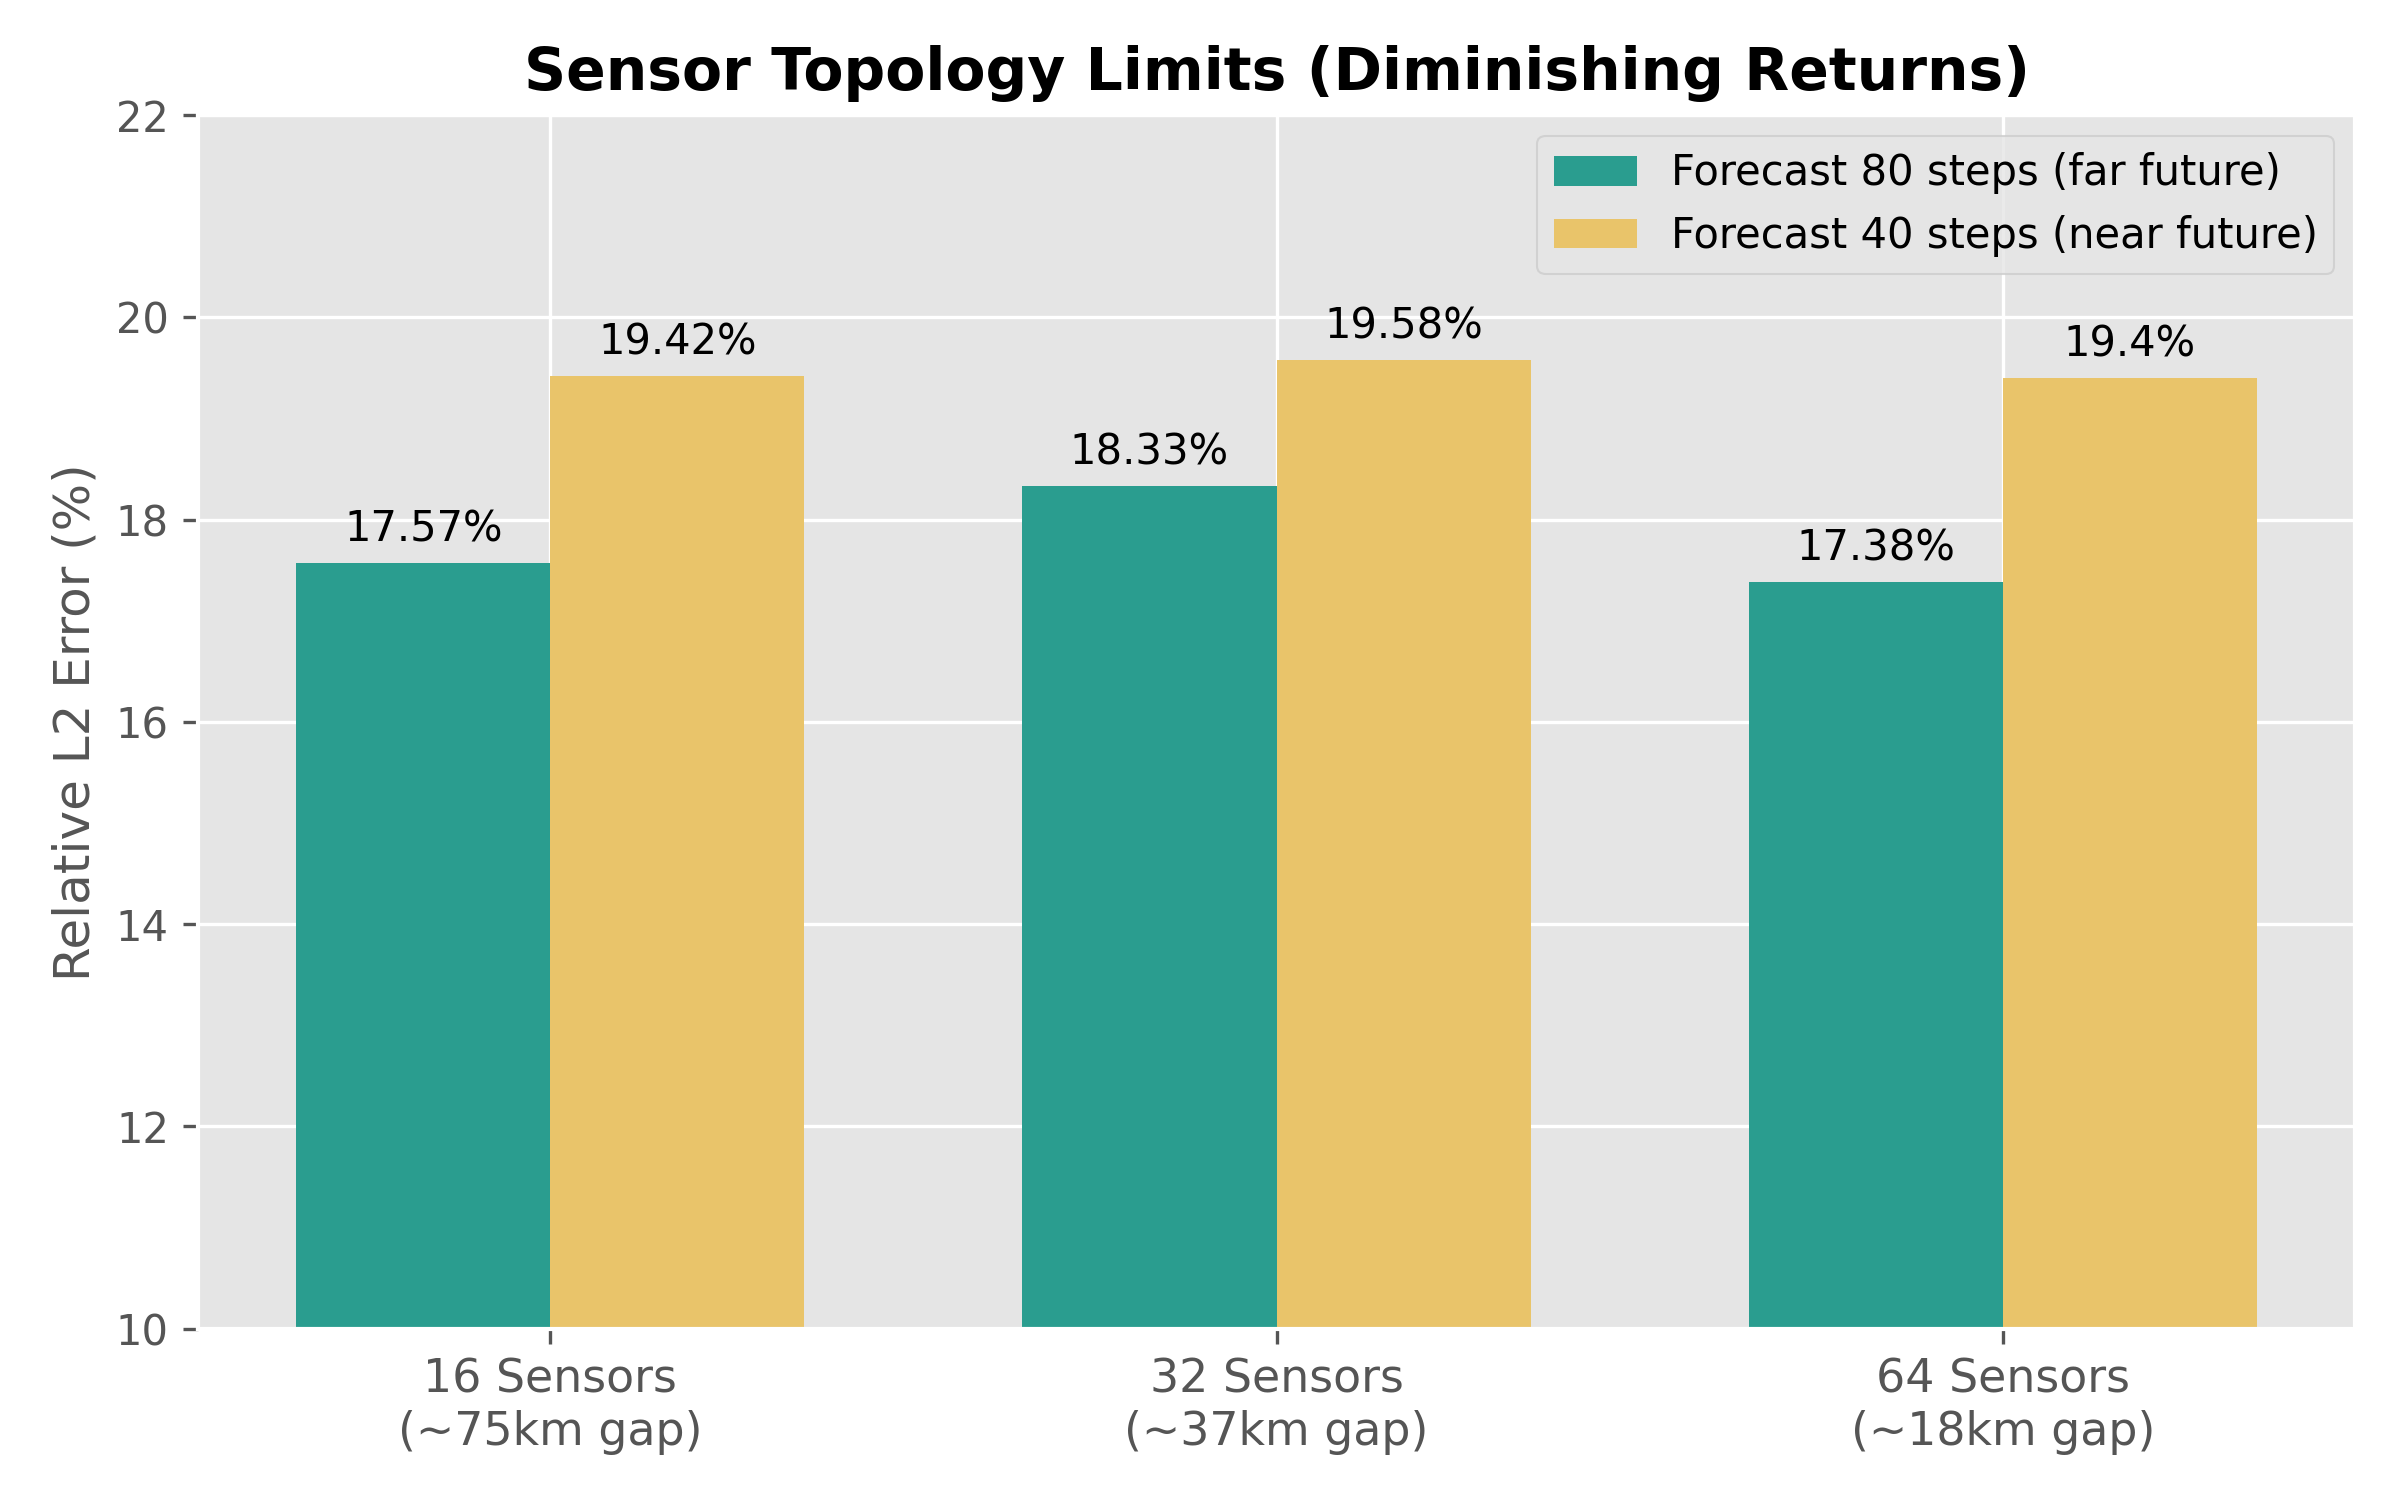
\includegraphics[width=0.72\linewidth]{figures/sensor_ablation.png}
    \caption{Effect of boundary sensor density on forecasting performance. Increasing the number of boundary sensors does not guarantee monotonic improvement when additional sensors are placed along the same boundary geometry. This diagnostic uses a separate synthetic long-horizon sensor-budget experiment and is not directly comparable to the mixed 1--24 h Copernicus benchmark.}
    \label{fig:sensor_ablation}
\end{figure}

These preliminary results suggest that increasing boundary sensor count alone may not guarantee monotonic improvement under fixed boundary placement geometry. A broader sensor-placement study with multiple configurations is needed to separate the effects of sensor count, placement, and induced observability structure. This motivates the learned observability approach of OVCNO, which adapts to the specific geometry at hand rather than assuming a fixed observability--count relationship.

\end{document}
